% From mitthesis package
% Version: 1.07, 2024/09/26
% Documentation: https://ctan.org/pkg/mitthesis


\lstdefinestyle{mystyle}{
    backgroundcolor=\color{CadetBlue!15!white},   
    commentstyle=\color{Red3},
    numberstyle=\tiny\color{gray},
    stringstyle=\color{Blue3},
    basicstyle=\small\ttfamily,
    breakatwhitespace=false,         
    breaklines=true,                 
    numbers=left,                    
    numbersep=5pt,                  
    showspaces=false,                
    showstringspaces=false,
    showtabs=false,                  
    tabsize=2,
    language=Python,
    basicstyle=\ttfamily,
	keywordstyle=\color{blue}\ttfamily,
	stringstyle=\color{red}\ttfamily,
    commentstyle=\color{green}\ttfamily,
    morecomment=[l][\color{magenta}]{\#}
}%
\lstset{language=Python,style={mystyle}}%

\lstdefinestyle{seudocode}{
    backgroundcolor=\color{Goldenrod!30!white},   
    commentstyle=\color{Red3},
    numberstyle=\tiny\color{gray},
    stringstyle=\color{Blue3},
    basicstyle=\small\ttfamily,
    breakatwhitespace=false,         
    breaklines=true,                 
    numbers=left,                    
    numbersep=5pt,                  
    showspaces=false,                
    showstringspaces=false,
    showtabs=false,                  
    tabsize=2,
    language=Python,
    basicstyle=\ttfamily,
	keywordstyle=\color{blue}\ttfamily,
	stringstyle=\color{red}\ttfamily,
    commentstyle=\color{green}\ttfamily,
    morecomment=[l][\color{magenta}]{\#}
}%


\chapter{Problemas comunes}
\label{problemasComunes}

En este capítulo se enumeran problemas comunes en el desarrollo de software embebido de control, extraídos principalmente del libro ``\textit{Design Patterns for Embedded Systems in C: An Embedded Software Engineering Toolkit}'' \cite{douglass}. Cabe recordar que, si bien el título del libro indica que propone patrones de diseño, las soluciones que presenta no lo son realmente y, en algunos casos, resultan inadecuadas. Además, se analiza la solución de diseño propuesta en dicho libro y, a su vez, se aporta una alternativa desde la perspectiva de la Ingeniería del Software (\gls{IS}) enfocada en el diseño para el cambio. En muchos casos, se identifica la posibilidad de aplicar ciertos patrones de diseño descritos en \cite{Gamma:1995:DPE:186897}, mientras que en otros se utilizan conceptos y metodologías clave del diseño para el cambio, propuestos por David L. Parnas \cite{Parnas02, Parnas1972, parnas1977abstract}.


\minitoc



\section{Acceso al hardware}
\label{Accesoalhardware}
Una de las características distintivas de los sistemas embebidos es que trabajan directamente con dispositivos de hardware. Cada uno de estos tiene sus propios protocolos de comunicación y estándares de funcionamiento (por ejemplo, direcciones de memoria, codificación de bits, etc), por lo tanto el software se debe ajustar a sus requerimientos. Como se puede entender esta tarea no es simple y puede demandar mucho esfuerzo cada vez que se quiera modificar o agregar un componente de hardware. A su vez, puede que múltiples módulos de un sistema embebido quieran acceder al dispositivo, por lo que cada uno debe encargarse de la comunicación creando código repetido y complicando aún más las modificaciones. 

Para entender los inconvenientes que puede conllevar no diseñar pensando en el cambio se trabajará sobre un ejemplo simple. Suponga que se tiene un sistema embebido que debe controlar un motor de corriente continua (\gls{DC}) y que el software para hacerlo corre en un \gls{MCU} de la empresa \gls{arduinoEmpre}. Los requerimientos definen que es necesario poder asignar el sentido de giro (horario o antihorario) y la velocidad de rotación del motor según se necesite. Para controlar el motor se utiliza una placa \gls{DRV8838}, la cual se coloca entre el \gls{MCU} y el motor. Es necesario ya que el microcontrolador y su plataforma no pueden manejar las potencias requeridas para hacer funcionar el dispositivo. Podemos ver el conexionado de la mismo en la Figura \ref{drv8838}.

\begin{figure}[h]
    \centering
    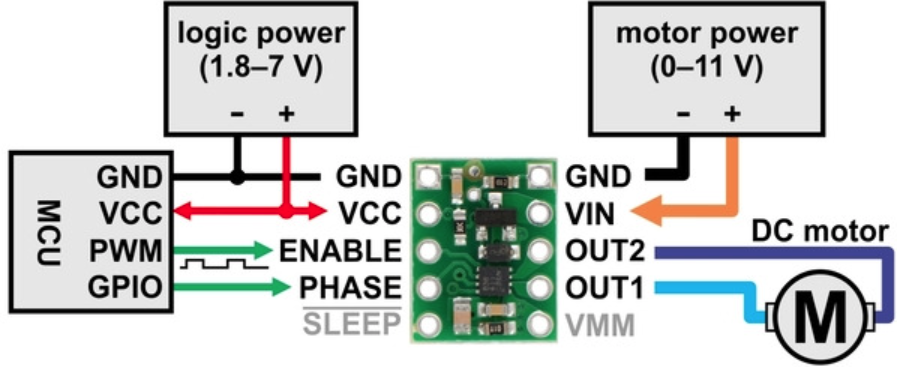
\includegraphics[width=0.65\linewidth]{drv8838.png}
    \caption{Conexionado de la placa de control DRV8838.}
    \label{drv8838}
\end{figure}

Como se observa la placa \gls{DRV8838} tiene múltiples pines. De estos podemos identificar dos grupos: los que aparecen a la izquierda, que llamaremos pines de entrada, y los de la derecha, que denominaremos pines de salida. El \gls{MCU} se conecta a los pines de entrada y, a través de estos, controlará el funcionamiento de la placa. En cambio, en los pines de salida se conecta el motor y transmiten la potencia necesaria.

Dentro de cada uno de estos grupos se encuentran pines destinados a la comunicación entre componentes, y otros que se utilizan para alimentar tanto la lógica de la placa \gls{DRV8838} como al motor. Estos últimos son \textit{GND}, \textit{VCC} y \textit{VIN}. Los pines de control de entrada son \textit{ENABLE}, \textit{PHASE} y \textit{SLEEP}, aunque en este ejemplo se utilizarán solo los dos primeros para simplificar la explicación. De todas formas, en la Tabla \ref{funciones_pin_drv8838} se puede consultar la función de cada pin y si la señal correspondiente es analógica o digital. Por último, \textit{OUT1}, \textit{OUT2} y \textit{VMM} son los pines de salida hacia el motor, y son los que finalmente transmiten la tensión y potencia necesarias para lograr el comportamiento deseado del motor.

\begin{table}[h]
\centering
\begin{tabular}{lllll}
\cline{1-3}
\multicolumn{1}{|l|}{PHASE}  & \multicolumn{1}{l|}{dirección de rotación} & \multicolumn{1}{l|}{digital}   &  &  \\ \cline{1-3}
\multicolumn{1}{|l|}{ENABLE} & \multicolumn{1}{l|}{velocidad de rotación} & \multicolumn{1}{l|}{analógico} &  &  \\ \cline{1-3}
\multicolumn{1}{|l|}{SLEEP}  & \multicolumn{1}{l|}{liberar fuerza}        & \multicolumn{1}{l|}{digital}   &  &  \\ \cline{1-3}
                             &                                            &                                &  & 
\end{tabular}
\caption{Funciones de cada pin del módulo DRV8838}
\label{funciones_pin_drv8838}
\end{table}

\gls{MCU} se conecta a los pines de \textit{ENABLE}, \textit{PHASE} y \textit{SLEEP} el software deberá gestionarlos. Pero, como se mencionó, para acotar el ejemplo se restringieron los requerimientos y para complirlos solo necesitaremos trabajar con los pines \textit{ENABLE} y \textit{PHASE}. Tendremos entonces dos cables conectados desde \gls{microcontrolador} a la placa \gls{DRV8838}, uno que se dirige a \textit{ENABLE} y otro a \textit{PHASE}. En el pseudo-código \ref{listing1} se encuentran las lineas necesarias para poder configurar el motor para luego poder utilizarlo en el resto del sistema. En estas se establece que el pin número siete del \gls{MCU} está conectado a el pin \textit{PHASE} y que el nueve a \textit{ENABLE}. Y a su vez se inicializa el pin dentro del software como pin de salida (\textit{OUTPUT}). Esto es necesario para que otras funciones que se llamen en el futuro se comporten como esperamos.

\begin{lstlisting}[caption=Configuración inicial del control del motor DC.,label={listing1}]
# Notar que los numeros asignados a los pines son arbitrarios dentro del conjunto de pines disponibles en nuestro Arduino.

# Constantes globales
DIR_pin = 7
VEL_pin = 9

def setup()
     .
     .
     .
  pinMode(DIR_pin, OUTPUT)
  pinMode(VEL_pin, OUTPUT)
     .
     .
     .
\end{lstlisting}


Una vez configurados los pines podemos hacer uso de las funciones \verb|pinMode|, \verb|digitalWrite| y \verb|analogWrite| provistas por el entorno de desarrollo de Arduino. Sus nombres son bastastantes descriptivos de su comportamiento, \verb|pinMode| configura el modo de operacion de un PIN en particular, puede ser \verb|OUTPUT| o \verb|INPUT| (entrada o salida). Y tanto \verb|digitalWrite| como \verb|analogWrite|, configuran en un PIN el valor especificado. \verb|digitalWrite| admite dos valores definidos por el entorno \verb|HIGH| y \verb|DOWN|. Por lo tanto, si se quiere establecer la máxima velocidad de giro en el motor se haría algo como en el Código \ref{codigoMax}. Y en caso de querer detenerlo usamos \verb|analogWrite| de la forma que se muestra en el Código \ref{codigoDet}.

\begin{lstlisting}[caption=Establecer 
máxima velocidad giro en sentido horario.,label={codigoMax}]
digitalWrite(DIR_pin, HIGH)
analogWrite(VEL_pin, 255) # Maximo valor aceptado, PWM siempre encendido
\end{lstlisting}

\begin{lstlisting}[caption=Detener giro del motor DC., label={codigoDet}]
analogWrite(VEL_pin, 0)
\end{lstlisting}

No es necesario entender por completo qué hace cada llamada, pero sí es importante comprender que ejecutar el Código \ref{codigoMax} y \ref{codigoDet} es fundamental para controlar el motor. Es decir, cualquier cliente del motor en el sistema debe saber que, para hacer que el motor gire a la máxima velocidad, es necesario ejecutar las dos lineas mostradas en el Código \ref{codigoMax} sobre los pines correspondientes al motor. Por ejemplo, si se desea realizar una acción con el motor en función del valor de alguna variable del sistema (\verb|valor|), \textbf{tradicionalmente} se implementa algo similar al código mostrado en el Código \ref{listingMotor}. En el cual si se cumple la condición de que \verb|valor| es mayor a 100 se ordenará al motor que avance a máxima velocidad, en caso contrario se indicará velocidad nula.

\begin{lstlisting}[caption=Ejemplo uso del motor DC.,label={listingMotor}]
def controlar_motor()

	if (valor > 100)
    	digitalWrite(DIR_pin, HIGH)
	    analogWrite(VEL_pin, 255)
	else
	    analogWrite(VEL_pin, 0)

\end{lstlisting}

¿Qué problemas tiene esta estrategia de cara al cambio?
\begin{itemize}
	\item Consideremos un caso en el que un segundo motor es agregado. Este es controlado por otra placa \gls{DRV8838} que también se conecta con dos pines al \gls{MCU}. Para poder utilizarlo en el código debemos definir al, al igual que con el primer motor, los dos pines que utilizará, supongamos en este caso \verb|DIR_pin2| y \verb|VEL_pin2|. Si queremos modificar la función \verb|controlar_motor| para incluir a este nuevo motor podríamos hacer algo como en el Código \ref{motor2}.
	
\begin{lstlisting}[caption=Extención de la función controlar\_motor para controlar dos motores.,label={motor2}]
def controlar_motor(motor)

	if (valor > 100)
		if (motor = IDMotor1)
    		digitalWrite(DIR_pin, HIGH)
	    	analogWrite(VEL_pin, 255)
	    else if (motor = IDMotor2)
	    	digitalWrite(DIR_pin2, HIGH)
	    	analogWrite(VEL_pin2, 255)
	    	.
	    	.
	    	.
	else
		if (motor = IDMotor1)
	    	analogWrite(VEL_pin, 0)
	    else if (motor = IDMotor2)
	    	analogWrite(VEL_pin2, 0)
	    	.
	    	.
	    	.

\end{lstlisting}
	
La modificación consiste en verificar que motor es el que se quiere manipular y en base a eso enviar la señal a traves de los pines correspondientes. Pero, ¿qué pasaría si se quiere añadir un tercer motor? Deberíamos agregar aún mas sentencias \verb|if else|, extendiendo aun más el código. ¿Y si debemos realizar operaciones diferentes según cada motor? Por ejemplo, en el caso que \verb|valor| sea mayor a 100 con el motor 1 se debe establecer velocidad máxima pero con el motor 2 nula. El cambio en el código es pequeño (ver Código \ref{motor2mod}), solo cambia un valor en la linea 9. Pero introduce complejidad en la lectura y comprensión facilitando la introducción de errores en futuras modificaciones. Es insostenible en el tiempo este enfoque de diseño.
\begin{lstlisting}[caption=Modificación de la función controlar\_motor para cambiar comportamiento al utilizar el motor 2.,label={motor2mod}]
def controlar_motor(motor)

	if (valor > 100)
		if (motor = IDMotor1)
    		digitalWrite(DIR_pin, HIGH)
	    	analogWrite(VEL_pin, 255)
		else if (motor = IDMotor2)
	    	digitalWrite(DIR_pin2, HIGH)
	    	analogWrite(VEL_pin2, 0)
	    	.
	    	.
	    	.
	else
		if (motor = IDMotor1)
	    	analogWrite(VEL_pin, 0)
		else if (motor = IDMotor2)
	    	analogWrite(VEL_pin2, 0)
	    	.
	    	.
	    	.

\end{lstlisting}
	\item Imagine el caso en el que por cierto motivo se debe invertir el sentido de giro del motor, de manera que lo que era ir giro horario ahora es anti horario. Para llevar a cabo el cambio, debemos modificar \textbf{todas} las llamadas a \verb|digitalWrite(DIR_pin, HIGH)|, tanto en el código que de la función \verb|controlar_motor| como en el resto del sistema, cambiando \verb|HIGH| por \verb|DOWN| y viceversa. Por ejemplo, en el Código \ref{motor2mod} debemos modificar las lineas 5 y 8. Es fácil cometer un error y dejar al sistema en un estado inconsistente. Ni hablar en el caso que se planteó en el punto anterior, puede ser necesario discriminar entre motores. La precaución a la hora de modificar debe ser mayor aún y a su vez la probabilidad de introducir errores aumenta.
   
    \item Por cierto motivo se descompuso la placa controladora del motor 1, y no se consigue un reemplazo idéntico, sino que se adquiere una nueva placa de otra marca, por ejemplo, una \textit{Pololu Simple Motor Controller G2}. En este caso, este placa no utiliza la misma interfaz de control que el \gls{DVR8838}, sino para controlarla se accede a ella mediante comunicación serial (utiliza un solo pin especifico). Incluso utilizando las herramientas provistas por el entorno de \gls{arduino}, el nuevo código de configuración (ver Codigo \ref{listingDistinto}) y uso (ver Codigos \ref{maxSerial} y \ref{detSerial}) difiere significativamente del anterior (Codigo \ref{listing1} para configuración y Codigos \ref{codigoMax} y \ref{codigoDet} para uso).
\begin{lstlisting}[caption=Configuración de la placa de control del motor DC utiliza comunicación serie., label={listingDistinto}]
def set_up() 
    .
    .
    .
    Serial.begin(9000)
    .
    .
    .

    \end{lstlisting}
\begin{lstlisting}[caption=Establecer máxima velocidad giro horario para el caso de comunicación en serie., label={maxSerial}]
Serial.write(0xAA)
Serial.write(0x0C)
Serial.write(0x85)
Serial.write(0x7F)
\end{lstlisting}
\begin{lstlisting}[caption=Establecer detención para el caso de comunicación en serie., label={detSerial}]
Serial.write(0xAA)
Serial.write(0x0C)
Serial.write(0xE0)
\end{lstlisting}
    Por lo tanto debemos modificar todos los usos de la antigua implementación por la nueva, lo cual además requerir un esfuerzo considerable, da pie a errores y obliga a reverificar código que ya se sabía que funcionaba correctamente. Se debe modificar las lineas 5, 6 y 15 de la función \verb|controlar_motor| de la manera mostrada en el Código \ref{motor1serial}.

\begin{lstlisting}[caption=Modificación de la función controlar\_motor para utilizar placa de control serial para controlar el motor 1.,label={motor1serial}]
def controlar_motor(motor)

	if (valor > 100)
		if (motor = IDMotor1)
    		Serial.write(0xAA)
				Serial.write(0x0C)
				Serial.write(0x85)
				Serial.write(0x7F)
		else if (motor = IDMotor2)
				digitalWrite(DIR_pin2, HIGH)
	    	analogWrite(VEL_pin2, 0)
	    	.
	    	.
	    	.
	else
		if (motor = IDMotor1)
	    	Serial.write(0xAA)
				Serial.write(0x0C)
				Serial.write(0xE0)
		else if (motor = IDMotor2)
	    	analogWrite(VEL_pin2, 0)
	    	.
	    	.
	    	.

\end{lstlisting}

Pero... ¿y si en el futuro se consigue la placa \gls{DRV8838}? Muchas veces se suele añadir una bandera que indique el tipo de hardware. En este caso, se podría definir una constante, por ejemplo, \verb|TIPO_MOTOR1|, que identifique el tipo de placa controladora. Al incorporar esta bandera en nuestra función \verb|controlar_motor|, se obtiene el Código \ref{motorBandera}.

\begin{lstlisting}[caption=Modificación de la función controlar\_motor para utilizar bandera indicadora de tipo de placa controladora.,label={motorBandera}]
def controlar_motor(motor)

	if (valor > 100)
		if (motor = IDMotor1)
			if (TIPO_MOTOR1 = DVR8838):
			    digitalWrite(DIR_pin, HIGH)
	    		analogWrite(VEL_pin, 255)
			else if (TIPO_MOTOR1 = Pololu):
    			Serial.write(0xAA)
					Serial.write(0x0C)
					Serial.write(0x85)
					Serial.write(0x7F)
		else if (motor = IDMotor2)
	    	digitalWrite(DIR_pin2, HIGH)
	    	analogWrite(VEL_pin2, 0)
	    	.
	    	.
	    	.
	else
		if (motor = IDMotor1)
			if (TIPO_MOTOR1 = DVR8838):
				analogWrite(VEL_pin1, 255)
			else if (TIPO_MOTOR1 = Pololu):
	    	Serial.write(0xAA)
				Serial.write(0x0C)
				Serial.write(0xE0)
	    else if (motor = IDMotor2)
	    	analogWrite(VEL_pin2, 0)
	    	.
	    	.
	    	.

\end{lstlisting}

Esto no es una buena solución, ya que lo unico que logra es generar más dificulad a la hora de introducir un nuevo cambio. Ahora, si se debe cambiar la lógica de la función, debemos tener en cuenta más lineas a modificar. Introduciendo así más posibilidades de cometer errores.

    \item Claramente, el código obtenido es poco claro; es decir, no resulta fácil comprender de qué se trata una determinada porción de código con solo leerla. Basta con intentar entender la función del Código \ref{motorBandera} para comprobarlo. A su vez, el código resulta difícil de modificar, ya que requiere un esfuerzo adicional de comprensión antes de poder aplicar cualquier cambio. En el ejemplo, la lógica principal de la función es sencilla —solo una sentencia condicional—, pero en general las funciones suelen ser más complejas e incluyen múltiples sentencias, estructuras anidadas y bucles.


\end{itemize}

En el libro, la solución de este problema es nombrada como un patrón de diseño, el patrón \textit{``Hardware Proxy''}. Pero desde el punto de vista de la IS, no es un patrón de diseño, sino uno de los principios fundamentales de la  IS, que es el \gls{dboi}.

\declareCMod{MotorDC}

Estos inconvenientes son derivados de que el \textit{hardware} comprende un ítem de cambio frecuente; por lo que si seguimos la metodología de Parnas (ver sección \ref{metoParnas}), se debe aislar ese posible cambio en un módulo. En el ejemplo que se está trabajado, se debe crear un módulo que encapsula el hardware en cuestión, el motor \gls{DC}. Este módulo oculta cómo debe ser usado el hardware y provee una interfaz lo suficientemente insensible a la implementación. Es decir, al momento de confeccionar la interfaz del módulo se debe pensar en lo que el motor siempre va a hacer independientemente de los posibles cambios que sufra el hardware subyacente. Para esto, se debe elegir la cantidad de mínima de métodos del modo más abstracto posible, sin agregar métodos que puedan ser reemplazados utilizando otros que ya fueron definidos \cite{Parnas02, parnas1977abstract}.
Un motor \gls{DC} siempre recibirá ordenes para definir su sentido y velocidad de rotación. La Figura \ref{interfazMotor} presenta la interfaz del módulo \MotorDC que encapsula el hardware relacionado al motor.

\begin{figure}[H]
\caption{Interfaz MotorDC}
\label{interfazMotor}
\begin{center}
\begin{tikzpicture}\sf
\umlclass[x=-3]{MotorDC}
{
MotorDC(i: Pin, i: Pin)
}
{
    
    setDir(i: Dir) \\ 
    setVel(i: Vel) \\
}
\end{tikzpicture}
\end{center}
\end{figure}

Si se cuenta con dos o mas motores del mismo tipo, se crearán dos a mas instancias del módulo. Para esto el contrsuctor recibirá como parámetros los pines de control, el método de \verb|setDir| toma el valor de dirección a establecer y el input de \verb|setVel| el valor de velocidad deseado. En el Código \ref{constructorMotor} se puede ver un ejemplo de una posible implementación de esta interfaz utilizando el controlador \gls{DVR8838}.

\begin{lstlisting}[caption=Posible implementación de la interfaz del módulo MotorDC.,label={constructorMotor}]
def MotorDC(dir_pin, vel_pin);
    pinMode(this.dir_pin, OUTPUT)
    pinMode(this.vel_pin, OUTPUT)


def setDir(dir) 
    if (dir == HORARIO)
        digitalWrite(dir_pin, HIGH)
    else
        digitalWrite(dir_pin, DOWN)
        

def setVel(vel)
    analogWrite(vel_pin, vel)

\end{lstlisting}

En el código \ref{ejeploUsoMotor} se evidencian las primeras ventajas, el uso del motor en el código es mucho más claro en comparación al diseño tradicional, donde teniamos que escribir las lineas de los Códigos \ref{listing1} y \ref{codigoMax} para lograr lo mismo.

\begin{lstlisting}[caption=Ejemplo de uso de la interfaz del módulo MotorDC, label={ejeploUsoMotor}]
motor = MotorDC(1, 2)

motor.setDir(Dir.HORARIO)
motor.setVel(255)
\end{lstlisting}

Además, si se debe invertir el sentido de giro como en el ejemplo propuesto al comienzo de la sección, es tan fácil como cambiar la implementación del método \verb|setDir|, los clientes no notarán el cambio. A su vez, si se quiere controlar otro motor es posible hacerlo fácilmente como en el Código \ref{ejemploOtroMotor}. 

\begin{lstlisting}[caption=Ejemplo control nuevo motor DC.,label={ejemploOtroMotor}]
motor_delantero = MotorDC(18, 19)

motor_delantero.setDir(ANTIHORARIO)
motor_delantero.setVel(10)
\end{lstlisting}


En caso de un cambio de componente de hardware, como el explicado anteriormente, los clientes del módulo no lo notarán, dado que la interfaz se mantendrá intacta. Por ejemplo, para el motor que utiliza comunicación serie, \verb|setDir| será redefinida como en el código \ref{nuevaSetDir} teniendo que solo volver a verificar el módulo \MotorDC.

\begin{lstlisting}[caption=Implementación método setVel para el motor que utiliza comunicación serie.,label={nuevaSetDir}]
def setVel(vel)
        serial.write(0xAA;
        serial.write(0x0C)
        hex_vel = int_to_hex(vel)
        serial.write(hex_vel)
\end{lstlisting}

Sin embargo, haciendo uso del concepto de herencia de interfaz y la noción de abierto-cerrado (explicados en la sección \ref{ingso}). Esto permite reutilizar módulos ya implementados y abstraer aún más la implementación. Para hacerlo se define un módulo abstraco \textit{\MotorDC} del cual hereda la interfaz cada modelo o combinación de motor y placa controladora. ELa Figura \ref{estructuraHerencia} presenta la estructura de interfaces de esta solución.

\begin{figure}[H]
\caption{Módulo MotorDC abstracto y estructura de herencia.}
\label{estructuraHerencia}
\begin{center}
\begin{tikzpicture}\sf
\umlclass[x=0,type=abstract]{MotorDC}
{}
{
    \umlvirt{setDir(i: Dir)} \\ 
    \umlvirt{setVel(i: Vel)} \\
}

\umlclass[x=-3, y=-4]{MotorDCDVR8838}
{
	MotorDC(i: Pin, i: Pin)
}
{
    setDir(i: Dir) \\ 
    setVel(i: Vel) \\
}
\umlclass[x=3, y=-4]{MotorDCG2}
{
	MotorDC(i: Serial)
}
{
    setDir(i: Dir) \\ 
    setVel(i: Vel) \\
}
\umlinherit[geometry=|-|]{MotorDCDVR8838}{MotorDC}
\umlinherit[geometry=|-|]{MotorDCG2}{MotorDC}
\end{tikzpicture}
\end{center}
\end{figure}

El cliente solo sabe que manipula un elemento \textit{\MotorDC}, no tiene noción con cual de los dos tipos de de placa controladora esta tratando. También es posible agregar más herederos, uno por cada modelo de placa controladora/motor, y reutilizar las módulos implementados en caso de utilizar hardware idéntico.

Siguiendo con el ejemplo de la función \verb|controlar_motor| veamos en la Figura \ref{motorEncapsulado} cómo es una posible implementación de esta misma utilizando la encapsulación del hardware propuesta. Con esta solución el codigo de la funcion no deberá ser modificado por más que cambien las marcas/tipos de placas controladoras.

\begin{lstlisting}[caption=Implementación de la función controlar\_motor utilizando encapsulación del hardware.,label={motorEncapsulado}]
def controlar_motor(motor: MotorDC)
	if (valor > 100)
		motor.setDir(HORARIO)
		motor.setDir(VelMaxima)
	else
		motor.setDir(VelNula)
\end{lstlisting}

De esta manera se siguen las prácticas recomendadas en la \gls{IS} \cite{ShawGarlan1996, ghezzi2003, bass2003, DBLP:books/daglib/0030743} y se obtiene un diseño orientado al cambio \cite{Gamma:1995:DPE:186897}.

\section{Interfaces que no se ajustan perfectamente}
Muchas veces el proveedor del hardware incluye con este librerías para su control, otras veces se consiguen en internet o se extraen de previos proyectos. Esto permite ahorrar tiempo de implementación, pero puede causar algunos inconvenientes si no se tiene en cuenta al cambio.

Tradicionalmente, se toman las librerías necesarias para controlar el hardware y se las utiliza directamente a lo largo del sistema. Lo que provoca que ante un cambio de hardware se debe modificar todos los usos de la librería con el nuevo código. Veamos un ejemplo en donde se evidenciará el inconveniente y cómo podemos anticiarnos al mismo.

Suponga el siguiente ejemplo: en un cierto sistema embebido se utiliza un display de 7 segmentos que forman un 8. Encendiendo o apagando independientemente cada segmento, se pueden mostrar distintos caracteres. Este display es de 4 dígitos y se emplea para mostrar la temperatura de funcionamiento y la posición, en grados, de cierto actuador, como se muestra en la figura \ref{fig:enter-label}.

\begin{figure}[h]
    \centering
    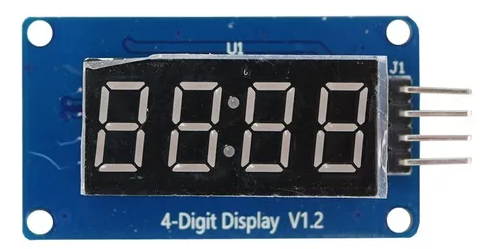
\includegraphics[width=0.5\linewidth]{display.png}
    \caption{Display 7 segmentos 4 digitos}
    \label{fig:enter-label}
\end{figure}

\declareCMod{LibAcme}
\declareCMod{LibEmca}

Este display recibe la información utilizando comunicación en serie, con un protocolo propio del fabricante. Para facilitar su uso, el fabricante brinda una librería llamada \LibAcme que implementa la comunicación y provee funciones simples de usar, tales como \verb|escribir(i: string): bool| y \verb|limpiar()|. La primera intenta escribir la cadena de caracteres indicada, pero solo lo hace si el display no está mostrando nada. En ese caso devuelve \verb|True| indicando que la acción fue completada con éxito. En caso contrario, es decir el display está mostrando texto al momento de llamar el método, retorna \verb|False|. \verb|limpiar()|, siempre limpia el display. Por lo tanto, se implementó el sistema utilizando las funciones provistas. Para comunicarse, múltiples módulos llaman esas funciones de la manera expuesta en el Código \ref{usoLibAcme}.

\begin{lstlisting}[label={usoLibAcme}, caption=Ejemplo de uso de la libreria LibAcme.]
libAcme = LibAcme()

if libAcme.escribir("24")
	print("El display estaba vacio, se pudo escribir el nuevo texto")
else
	print("El display esta ocupado mostrando algo, no se pudo escribir")

\end{lstlisting}

En cierto momento, el módulo display dejó de funcionar y fue reemplazado por otro de un fabricante distinto, el cual utiliza un protocolo de comunicación diferente. Al igual que en el caso anterior, la empresa provee una librería \LibEmca para utilizar el nuevo display. Sin embargo, la interfaz no es la misma que la anterior, e incluso algunos comportamientos también difieren.

Por ejemplo, en la primera librería, el método de escritura devolvía \verb|False| si se intentaba escribir mientras el display ya estaba mostrando información. En cambio, en la nueva implementación, si el display está mostrando algo, el nuevo texto lo sobrescribe de inmediato. No obstante, esta nueva librería proporciona un método adicional \verb|get_current(): string| que permite consultar el contenido que se está mostrando en el momento en que es invocado.

Tradicionalmente, para utilizar el nuevo display, se modifican todas las llamadas a las funciones de la librería anterior en todo el sistema, incorporando la nueva lógica. En nuestro ejemplo, el Código \ref{usoLibAcme} debe ser reemplazado por el Código \ref{usoLibEmca}. Si bien el cambio puede parecer superficial, es importante considerar que con cada modificación será necesario actualizar manualmente y reverificar \textbf{todos} los usos de la librería a lo largo del sistema.
\begin{lstlisting}[label={usoLibEmca}, caption=Ejemplo de modificaciones necesarias para adaptar la nueva librería.]
libEmca = LibEmca()

// Con EMCA

if libEmca.get_current() == ""
	libEmca.imprimir("Hola mundo!")
	print("El display estaba vacio, se pudo escribir el nuevo texto")
else
	print("El display esta ocupado mostrando algo, no se pudo escribir")


\end{lstlisting}

Además, este es un ejemplo simple; en el mundo real, los cambios pueden ser mucho más complejos en su lógica y de distinta naturaleza. Este diseño puede representarse como se muestra en la Figura \ref{configOri}: un módulo que constituye la librería del fabricante y otro que actúa como cliente de esta, es decir, el resto del sistema.


\begin{figure}[H]
\caption{Diseño tradicional del uso de la libreria del fabricante.}
\label{configOri}
\begin{center}
\begin{tikzpicture}\sf
\umlsimpleclass[]{Cliente}

\umlclass[right=1.5cm of Cliente]{LibAcme}
{}
{
escribir(i: string): bool  \\
limpiar()
}

\umluniassoc[]{Cliente}{LibAcme}


\umlnote[below left=0.5cm and 0.5cm of LibAcme, width=3cm]{LibAcme}{
Librería externa.
}


\end{tikzpicture}
\end{center}
\end{figure}

Este diseño presenta un fuerte acoplamiento entre el \Cliente y la \LibAcme, por lo que cualquier cambio en el hardware repercutirá en el resto del sistema, trayendo consigo todas las desventajas mencionadas tanto en este capítulo como en el anterior. Se podría decir que el principal problema radica en que no se siguió la metodología de diseño propuesta por Parnas \cite{Parnas1972}. El hardware representa un ítem con alta probabilidad de cambio, por lo tanto, debe ser encapsulado.

En el libro de Douglass \cite{douglass} se observa que, en la práctica, este tipo de escenarios son comunes: ya se tiene un sistema funcionando y se produce un cambio de hardware. Por ello, se intentará proponer una posible solución desde el punto de vista de la \gls{IS}. En lugar de reescribir todo el sistema, veremos cómo, aplicando un patrón de diseño de Gamma \cite{Gamma:1995:DPE:186897}, es posible adaptar el sistema y preparar el diseño del mismo para futuros cambios de índole similar.
\declareAMod{Display}
Para encapsular el hardware sin modificar todo el sistema se creará un módulo abstracto llamado \Display. En su interfaz proveerá los mismos métodos que \LibAcme de esta manera evitaremos cambiar la implementación del resto del sistema. Al compartir interfaz podemos decir que \LibAcme hereda la interfaz de \Display, esto lo podemos ver en la Figura {configUsando}.

\begin{figure}[H]
\caption{Introducción del nuevo módulo abstracto\Display.}
\label{configUsando}
\begin{center}
\begin{tikzpicture}\sf
\umlsimpleclass[]{Cliente}

\umlclass[right=1.5cm of Cliente,type=abstract]{Display}
{}
{
\umlvirt{escribir(i: string): bool}  \\
\umlvirt{limpiar()}
}

\umlclass[right=0.5cm of Cliente,below=2cm of Cliente]{LibAcme}
{}
{
escribir(i: string): bool  \\
limpiar()
}

\umluniassoc[]{Cliente}{Display}
\umlinherit[geometry=|-|]{LibAcme}{Display}


\end{tikzpicture}
\end{center}
\end{figure}
\declareCMod{DisplayEmca}
Como mencionamos, \LibEmca se utiliza para controlar el nuevo display, pero su interfaz y funcionalidad no son las mismas que las de \LibAcme. Por lo tanto, aplicaremos el patrón \textit{Adapter} (Adaptador) propuesto por Gamma \cite{Gamma:1995:DPE:186897}. Este patrón consiste, en este caso, en crear un módulo \DisplayEmca, que se encarga de adaptar la interfaz de \LibEmca a la de \Display. Es decir, utilizará los métodos de \LibEmca para implementar la funcionalidad esperada por los métodos de \Display. De esta manera, se obtiene la estructura de módulos mostrada en la Figura \ref{configNueva}.

\begin{figure}[H]
\caption{Diseño aplicando el patrón \textit{Adapter}.}
\label{configNueva}
\begin{center}
\begin{tikzpicture}\sf
\umlsimpleclass[x=-4.5,y=1]{Cliente}

\umlclass[x=0,y=1,type=abstract]{Display}
{}
{
\umlvirt{escribir(i: str): bool}  \\
\umlvirt{limpiar()}
}
\umlclass[x=-2.5,y=-3]{LibAcme}
{}
{
escribir(i: str): bool  \\
limpiar()
}
\umlclass[x=2.5,y=-3]{DisplayEmca}
{}
{
escribir(i: str): bool  \\
limpiar()
}
\umlclass[x=8,y=0.5]{LibEmca}
{}
{
imprimir(i: str)  \\
get\_current(): str
}
umluniassoc
\umlinherit[geometry=|-|]{LibAcme}{Display}
\umlinherit[geometry=|-|]{DisplayEmca}{Display}
\umluniassoc[]{Cliente}{Display}
\umluniassoc[geometry=-|-]{DisplayEmca}{LibEmca}

\umlnote[below=0.5cm of LibEmca, width=3cm]{LibEmca}{
Librería externa.
}
\end{tikzpicture}
\end{center}
\end{figure}

No olvidar que cada aplicación de un patrón de diseño debe ser seguida por su correspondiente documentación \textbf{2MIL}. En este caso se la presenta en la Figura \ref{docAdapter}.

\begin{figure}[H]
\caption{Documentación de la aplicación del patrón Adapter al ejemplo del display.}
\label{docAdapter}
\begin{pattern}[]{Adaptar nuevo controlador de display}{Algorithm}{idFigAlg}
\based{Adaptador (Adapter)}
\why{\textbf{Cambios previstos}: Se pueden agregar diferentes displays pero manteniendo una interfaz común.

\textbf{Funcionalidad}: En caso de agregar un nuevo display que provee una intefaz diferente a la utilizada en el sistema, se crea un módulo que la adapta para que corresponda a la usada.
}
\assigns
\is{Display}{Target}
\is{LibEmca}{Adaptee}
\is{DisplayEmca}{Adapter}
\end{pattern}
\end{figure}


En el Código \ref{codigoAdapter} se presenta un ejemplo de implementación del módulo \DisplayEmca. En este se utilizan los métodos provistos por la librería del fabricante, y se emula la interfaz de \Display. De este modo, se permite reemplazar el hardware sin necesidad de modificar ni reverificar ninguna otra parte del sistema.

\begin{lstlisting}[label={codigoAdapter}, caption=Ejemplo de implementación del módulo \ControlEmca]
escribir(string palabra)
    if (libEmca.get_current() != "")
        return false
	else
    	libEmca.imprimir(cadena)
    	return true

limpiar()
    libEmca.imprimir("")
\end{lstlisting}

Las ventajas de aplicar este patrón en esta situación particular en la cual se parte de un diseño \textbf{no} oriendatado al cambio son:

\begin{itemize}

\item Facilitar la sustitución de hardware: permite cambiar el display sin necesidad de modificar el código del cliente, reduciendo el impacto del cambio de hardware en el sistema.

\item Mantiener la coherencia en la interfaz: el cliente sigue interactuando con la misma interfaz abstracta (\Display), evitando la necesidad de modificar múltiples módulos en el sistema.

\item Minimizar el riesgo de errores: al encapsular las diferencias de implementación en el adaptador (\DisplayEmca), se reduce la posibilidad de introducir errores al modificar manualmente todas las llamadas en el código.

\item Mejorar la mantenibilidad: cualquier nuevo display con una librearía de control solo requiere la creación de un nuevo adaptador.

\item Se promueve la reutilización de código: la abstracción permite reutilizar la lógica del cliente sin importar qué display se use, evitando la duplicación de código y mejorando la modularidad.
\end{itemize}


\section{Obtención de información}
\label{obtInfo}

Generalmente una tarea importante que tienen los sistemas embebidos es recavar información proveniente de sensores. Existen diferentes formas en las que los sensores transmiten información al sistema. Algunos, por ejemplo un sensor de temperatura, establece en el pin en el que está conectado un valor de tensión, por lo que el sistema solo debe consultar el valor del pin. Otros, en cambio, se comunican mediante interrupciones; por ejemplo un sensor de efecto \gls{hall} genera una interrupción por cada detección de campo magnético. Por lo tanto, si lo estamos usando para calcular las \gls{RPM} de un componente giratorio, debemos llevar una cuenta de las interrupciones que generó en cierto periodo de tiempo y realizar una operación matemática. Evidentemente, es necesario que alguna porción de nuestro sistema se encargue de hacerlo y maneje las interrupciones generadas por el sensor. Algo similar pasa con otro tipos de dispositivos como joysticks, botones, etc.

Tradicionalmente, esta tarea se centraliza en un único módulo que provee dos métodos: uno encargado de manejar la interrupción, procesar y almacenar la información, y otro que se utiliza para acceder a ella. Al aplicar esta solución, se obtiene una estructura poco resiliente al cambio. Por ejemplo, si se modifican los cálculos para obtener el resultado deseado, es necesario modificar también la implementación del módulo, lo que da lugar a la posible introducción de errores. Asimismo, la manera de transmitir la información relacionada con la interrupción puede variar debido a modificaciones en el hardware (tipo o modelo del sensor, componentes mecánicos, etc.). En \gls{IS}, decimos que el módulo oculta más de un ítem de cambio y, como vimos previamente, esto no se ajusta a las prácticas recomendadas.

Además, en muchos casos ni siquiera se construye este módulo, sino que cada cliente del dispositivo se encarga de capturar y procesar los datos provenientes, lo que provoca que, ante cualquier cambio, deba modificarse el código en diferentes módulos a lo largo del sistema.

Es debido a las problemáticas mencionadas que resulta útil contar con una forma general de abordar este problema desde el punto de vista del diseño orientado al cambio. Para ello, tomaremos como referencia el trabajo realizado sobre el robot desmalezador en \cite{paperPomponio}, en el cual se empleó la estructura modular presentada en la Figura \ref{activo}, destinada a llevar a cabo las actividades necesarias para el uso de sensores que generan interrupciones en el sistema. Replicaremos esta estructura, siguiendola casi como si fuera un patrón de diseño.

\begin{figure}[H]
\caption{Estructura componentes para la lectura de un sensor activo.}
\label{activo}
\centering
\begin{tikzpicture}\hypertarget{fig:ConnectBufferToMCU}{}
%-------------Estilos para dibujar-----
\tikzstyle{módulo}=[minimum width=1cm,inner sep=2mm,above right,draw,align=center,minimum width=2cm, font=\bfseries]

\tikzstyle{supest}=[rounded corners=1.5mm, minimum width=2cm,inner sep=2mm,draw,text width=2cm]

\tikzstyle{componente}=[minimum width=2cm,inner sep=2mm,draw,text width=2cm]

\tikzstyle{nombre}=[inner sep=0mm, font=\bfseries]

\tikzstyle{pipe}=[-latex,thick,line width=4pt]

\tikzstyle{modExt}=[minimum width=1cm,inner sep=2mm,above right,draw, dotted,line width=2pt,align=center,minimum width=2cm,color=gray, font=\bfseries]

\tikzstyle{flechaFisica}=[-latex,snake=coil,segment aspect=0, red, thick];
%--------------------------

\node[módulo,fill=yellow!20](Pin){Dispositivo};

\node[módulo, above left=0.5cm and 2cm of Pin, fill=yellow!20](CountTime){Comando};

\draw[flechaFisica](Pin) -| (CountTime);

\node[módulo, above=1cm of CountTime, fill=yellow!20](CRpinCollector){Colector};

\draw[-latex](CountTime) edge (CRpinCollector);

\node[módulo, left=1cm of CRpinCollector, fill=yellow!20](CRBuffer){Computador};

\draw[-latex](CRBuffer) edge (CRpinCollector);

\node[módulo, below=5cm of CRBuffer, fill=yellow!20](BufferReader){Cliente};

\draw[-latex](BufferReader) edge (CRBuffer);

\node[nombre, below right = 1cm and -3cm of Pin, fill=yellow!20](ConnectBufferToMCU){};

\node[componente, fit=(Pin)(CountTime)(CRBuffer)(ConnectBufferToMCU)]{};

%%------------------------------Referencias------------

\node[módulo, below left=1cm and 1cm of BufferReader, fill=yellow!20](mod){nombre};
\node[right =0.5cm of mod](modDesc){módulo};

\node[right=4cm of modDesc](x1){};
\node[right=2cm of x1](x2){};
\draw[-latex](x1)--(x2);
\node[right=0.3cm of x2](llp){llamada a procedimiento};

\node[below=0.5cm of mod.south west](x1a){};
\node[below=0.5cm of mod.south east](x2a){};
\draw[flechaFisica](x1a)--(x2a);
\node[below right=-0.4cm and 0.3cm of x2a, text width=4cm](hand){llamada a procedimiento a partir de una interrupción física (handler)};

%
\node[supest, fit=(mod)(hand)(llp)]{};

\end{tikzpicture}
\label{fig:ConnectBufferToMCU}
\end{figure}

\declareCMod{Dispositivo}
\declareCMod{Colector}
\declareCMod{Computador}
\declareCMod{Comando}

En esta estructura se distinguen cuatro módulos principales: \Dispositivo, que encapsula el hardware asociado al dispositivo encargado de generar e introducir la interrupción. Este módulo cuenta con un manejador de interrupción configurado para invocar al comando encapsulado en el módulo \Comando cuando la interrupción es lanzada. Este último sigue el patrón de diseño \textit{Command} y ejecuta los métodos del módulo \Colector para registrar la información requerida sobre la interrupción (por ejemplo, el momento exacto en que ocurrió el evento o la cantidad de veces que sucedió). De este modo, podemos deducir que \Colector almacena la información ``cruda'' proveniente de la interrupción o del sensor. Finalmente, se encuentra el módulo \Computador, encargado de procesar la información cuando esta es solicitada. Para ello, lee los valores almacenados en \Colector y aplica cálculos o algoritmos que computan la información final aportada por el dispositivo. Un ejemplo de ello podría ser el cálculo de la velocidad de rotación de una rueda o la obtención de los inputs de un joystick.

A continuación se presenta un ejemplo de aplicación con el objetivo de analizar en mayor profundidad la estructura modular. Se considera un sensor de efecto \gls{hall} montado de manera tal que, al girar una rueda, imanes permanentes pasen cerca de este. De esta forma, el sensor puede utilizarse para medir la velocidad de rotación. En la Figura \ref{hall} se observa la variación de voltaje producida por el paso de los imanes frente al sensor. Cada vez que el dispositivo detecta un campo magnético, emite una interrupción que es gestionada por el módulo \Comando, el cual actúa como un comando y, por lo tanto, conoce qué funciones ejecutar dentro del módulo \Colector.

\begin{figure}[H]
    
    \caption{Ejemplo de la variación de voltaje producida por un sensor de efecto Hall al detectar un cambio del campo magnético. Cada pico de voltaje provoca que el microcontrolador genere una interrupción. Imagen extraída de \cite{disenioViejo2}.}
    \centering
    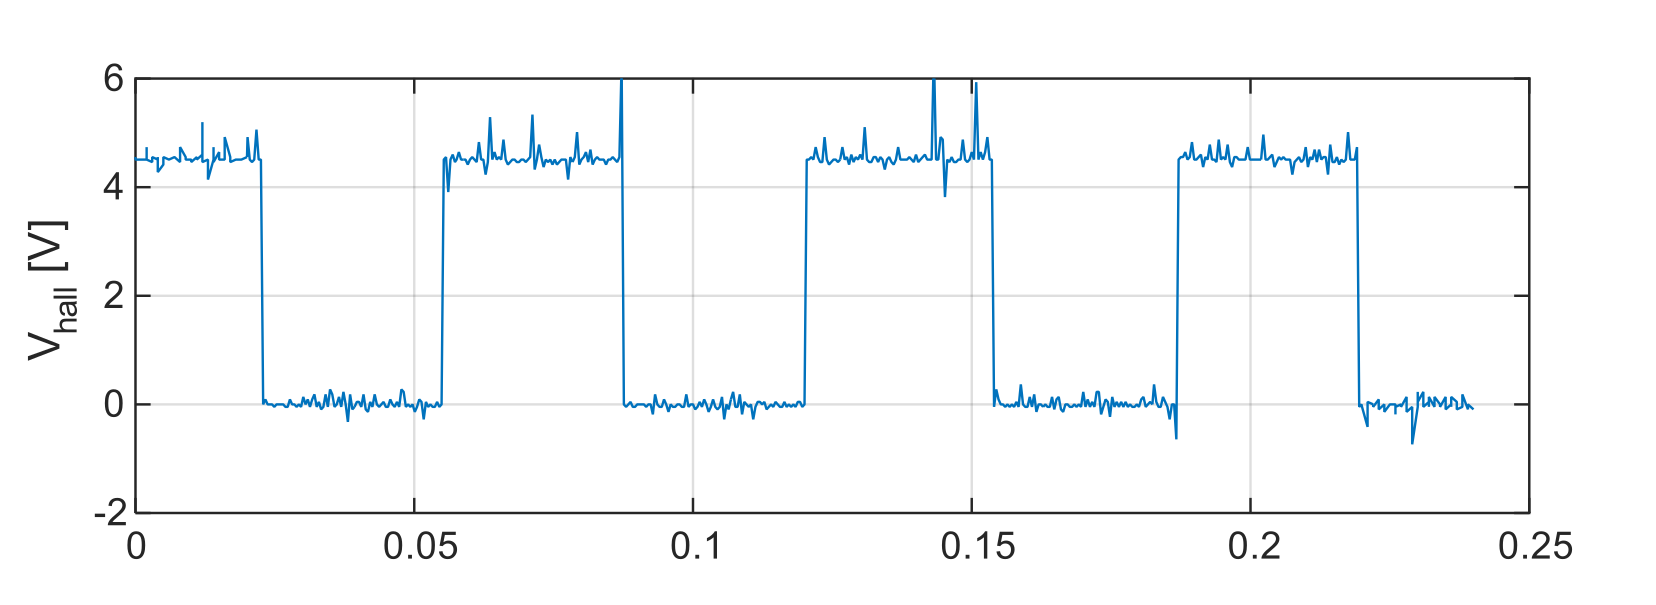
\includegraphics[width=0.8\linewidth]{sensorHall.png}
    \label{hall}
\end{figure}

\declareCMod{SensorVelocidad}

En la Figura \ref{estructuraHall} se presenta la estructura de módulos de esta solución, junto con pseudocódigo que ilustra una posible implementación.

Con los imanes colocados a una distancia conocida, para calcular la velocidad es necesario registrar los dos últimos instantes de tiempo en que fueron detectados. De forma simplificada, la velocidad se obtendrá al dividir la distancia entre los imanes por el tiempo transcurrido entre ambas detecciones. En consecuencia, el módulo \Colector debe proveer un método para almacenar el momento de cada detección. Posteriormente, el módulo \SensorVelocidad, que cumple la función de \Computador, tomará la información almacenada en \Colector y realizará el cálculo matemático para determinar la velocidad de giro de la rueda. Los cálculos, que pueden ser complejos, se ejecutarán únicamente bajo demanda, es decir, cuando el cliente lo requiera. Esto permite optimizar el rendimiento del sistema al disminuir la carga computacional necesaria. Cabe aclarar que este ejemplo está simplificado y omite situaciones que conllevarían una complejidad innecesaria.

\begin{figure}[H]
\caption{Ejemplo módulos para obtener la información referida a la velocidad.}
\label{estructuraHall}
\begin{center}
\scalebox{.90}{
\begin{tikzpicture}\sf

\umlclass[]{SensorHall}
{}
{
start()\\
stop()\\
signalHandler() \\
setCommand(i: Command)
}

\umlnote[above=1cm of SensorHall,width=3cm]{SensorHall}
{
signalHandler() \{\\
\ \ \ \ cmd.execute() \\
\}
}

\umlclass[above left=1cm and 2cm of SensorHall]{Count}
{}
{
execute() \\
}

\umlnote[below left=2.5cm and -1cm of Count,width=4cm]{Count}
{
Hereda de Command \\
execute() \{ \\
\ \ \ colector.addEvent() \\
\}
}

\umlclass[above=1cm of Count]{Colector}
{}
{
addEventTime() \\
getLastEventTime() \\
getSecondLastEventTime() \\
}

\umlclass[left=2cm of Colector]{SensorVelocidad}
{
Buffer(i: Collector)
}
{
getVelocidad()
}

\umlnote[below=1cm of SensorVelocidad,width=8cm]{SensorVelocidad}
{
getVelocidad() \{ \\
\ \ \ last = colector.getLastEventTime() \\
\ \ \ second = colector.getSecondLastEventTime() \\
\ \ \ return DISTANCIA / (last - second) \\
\}
}

\umlnote[right=1cm of Colector,width=5.5cm]{Colector}
{
addEventTime() \{ \\
\ \ \ secondLast = last \\
\ \ \ last = time.getCurrentTime() \\
\}

}

\umluniaggreg{SensorVelocidad}{Colector}
\umluniaggreg[geometry=-|]{SensorHall}{Count}

\end{tikzpicture}
}
\end{center}
\end{figure}

Al aplicar esta solución orientada al cambio, preparamos esta sección del sistema para cambios probables, tanto de hardware como de algoritmos. Además, las responsabilidades se separan en módulos independientes, logrando que una modificación en uno de ellos no afecte al resto del sistema. De este modo, si la rueda fuera modificada y cambiara la distancia entre los imanes, bastaría con actualizar la implementación del módulo \SensorVelocidad. A su vez, si el sensor \gls{hall} fuese reemplazado, solo se cambiaría el módulo que lo encapsula, manteniendo intacto el resto de la aplicación.

En esencia, las ventajas obtenidas con este diseño impactan directamente en la sostenibilidad y el ciclo de vida del software. Al lograr este nivel de bajo acoplamiento y alta cohesión, se minimiza el costo y el riesgo asociados al mantenimiento, ya que los cambios quedan confinados y son esperados. Esto no solo previene la propagación de errores, sino que genera que el sistema tenga una alta resiliencia y flexibilidad.


\subsubsection*{Recolectar información de manera periódica.}

Algunos sistemas se encargan de mostrar, almacenar o verificar la información de los sensores a intervalos regulares. En estos casos no resulta crítico perder valores intermedios, es decir, no se requiere una respuesta inmediata. Un ejemplo de ello puede ser una estación meteorológica o un dispositivo médico de monitorización, como un tensiómetro que registra los valores de presión del paciente cada cierto período.

Una implementación intuitiva consiste en escribir un \textit{loop} en el que se verifique la información de los sensores, llamando a métodos que la obtengan directamente del hardware, para luego ejecutar una función \textit{sleep} que bloquea el programa durante un tiempo determinado. Este enfoque presenta varias desventajas: en primer lugar, el tiempo de ejecución de la propia rutina alarga el período; en segundo lugar, si se desean agregar otras funcionalidades durante la espera, es necesario dividir la llamada a \textit{sleep} y recalcular los tiempos de ejecución.

Una solución más adecuada desde el punto de vista del diseño orientado al cambio es la siguiente: se configura un temporizador para que, cada \textit{x} cantidad de tiempo, genere una interrupción. Esta es una funcionalidad provista por muchos entornos de desarrollo para sistemas embebidos, como \gls{arduino}.
Para dicha interrupción, se registrará un \textit{handler} que consistirá en un módulo implementado según el patrón de diseño \textit{Command} (ver Sección \ref{patronCommand} para mas información sobre este tipo de aplicación del patrón). Este encapsula las funciones que deben ejecutarse para llevar a cabo la funcionalidad deseada como, por ejemplo, solicitar la información a sus respectivos módulos \Computador o a los sensores en sí, para luego registrarla en un cierto módulo que oculte la estructura de datos. De esta forma, se logra liberar al procesador durante los tiempos de espera y desacoplar esta funcionalidad.


\section{Máquinas de estado}\label{cap:state}

Muchos sistemas ajustan su comportamiento durante su ejecución en función de diversas causas, como interacciones con el entorno o requisitos internos. Un ejemplo sencillo es un sistema de control de microondas, que no iniciará el calentamiento si la puerta está abierta. En este caso, la condición de la puerta representa un estado interno que restringe un comportamiento (calentar) mientras permite otro. Del mismo modo, el comportamiento de un motor en un robot está determinado por su estado de dirección, que puede ser ``giro horario'' o ``giro antihorario''. Otro ejemplo es un sistema en el que, al finalizar una operación, se cambia del estado trabajando al estado esperando, lo que también altera el comportamiento del sistema. De manera similar, un sistema de climatización puede estar en estado calentando o enfriando, dependiendo de la configuración del termostato. Por lo tanto, la gestión de estados, sus transiciones y los cambios de comportamiento asociados a estos son aspectos fundamentales en el diseño de sistemas complejos y representan un item de cambio bastante probable.

Una solución de implementación tradicional para gestionar estados consiste en almacenarlos en una variable. Posteriormente, se verifica el valor de esta variable para modificar el comportamiento de las funciones, como se ilustra en el código \ref{codigoMicro}.

\begin{lstlisting}[label=codigoMicro,caption={Ejemplo de manejo de estados tradicional, en el caso del microondas.}]
calentar():
    if (estado == PuertaAbierta):
        return
    else if (estado == Preparado):
        magnetron.encender()
    else if (estado == Pausa):
    	magnetron.encender()

\end{lstlisting}

Este enfoque, si bien es directo, presenta varias desventajas al modificar o extender el código. Por ejemplo, al agregar nuevos estados o cambiar el comportamiento del sistema, la gestión se vuelve rápidamente compleja. Esta creciente complejidad es una de las principales desventajas de su implementación. A medida que se añaden más estados, cada método requiere más verificaciones, lo que conduce a una proliferación de estructuras \textit{if-else}. Esto no solo dificulta la lectura del código, sino que también aumenta la probabilidad de introducir errores, ya que cada nuevo estado debe ser cuidadosamente incorporado y verificado en todas las partes relevantes del sistema. Además, este enfoque compromete la sostenibilidad del software. En el Código \ref{nuevoEstado} se muestra cómo se agrega un nuevo estado al método \verb|calentar()|.

\begin{lstlisting}[label=nuevoEstado,caption={Ejemplo de introducción de un nuevo estado a la solución tradicional.}]
calentar():
    if (estado == PuertaAbierta):
        return
    else if (estado == Preparado):
        magnetron.encender()
    else if (estado == Pausa):
    	magnetron.encender()
    else if (estado == Calentando):
    	magnetron.apagar()

\end{lstlisting}

Cuando el comportamiento de un estado debe cambiar, es posible que se necesiten modificaciones en múltiples métodos. Esto puede llevar a la duplicación de código o dificultar la identificación de las partes que requieren cambios, complicando el proceso y aumentando el riesgo de errores. 

Otra desventaja clave es la baja modularidad, ya que el comportamiento asociado a cada estado no está claramente delimitado. Si cada estado requiere comportamientos complejos, el código se vuelve monolítico y difícil de extender sin alterar los métodos existentes. Por ejemplo, al agregar un estado ``EnPausa'', sería necesario modificar la lógica de múltiples métodos para verificar este nuevo estado y ajustar el comportamiento de manera apropiada. Todas estas deficiencias dificultan la reutilización del código y hacen que la verificación del correcto funcionamiento del sistema sea cada vez más compleja.

Este tipo de solución es ampliamente utilizado. Un ejemplo relevante se encuentra en el software original del robot desmalezador, como se describe en el informe \cite{informe1}. En particular, se definen diferentes estados de operación del robot y se utiliza una gran estructura de control \textit{switch-case} dentro del bucle principal. Esta estructura decide la acción a ejecutar en función del estado actual, como se detalla en el Código \ref{codigoLoopMain}.

\begin{lstlisting}[caption=Main loop del previo firmware del robot desmalezador \cite{informe1}, label={codigoLoopMain}]
switch (ESTADO) {
	case DUTY_REMOTO:
		duty_remoto();
		break;
	case RPM_REMOTO:
		rpm_remoto();
		break;
	case DUTY_PC:
		duty_pc();
		break;
	case RPM_PC:
		rpm_pc();
		break;	
	case CALIBRACION:
		calibracion();
		break;
	case PERDIDA_SENAL:
		perdida_senal();
		break;
	case EMERGENCIA:
		EMERGENCY();
		break;
	default:
		ESTADO = PERDIDA_SENAL;
		break;
}
\end{lstlisting}

Antes de abordar una perspectiva de diseño para gestionar el cambio, se analizará en detalle el ejemplo presentado en el libro de Douglass \cite{douglass} y la aplicación de una otra solución al manejo de estados.

El ejemplo propuesto consiste en el sistema de control de un microondas. Para representar el comportamiento del mismo, el autor presenta una máquina de estados como la de la Figura \ref{maquinaMicroondas}. Aunque contiene algunas incoherencias y no es del todo exacta, es suficiente para el propósito del ejemplo que se busca exponer.

\begin{figure}[h]
\caption{Máquina de estados extraída del libro \cite{douglass}.}
\label{maquinaMicroondas}
\begin{center}
\begin{tikzpicture}

\umlsimpleclass[fill=red!20, x=-3]{Apagado}
\umlsimpleclass[fill=red!20, x=3]{Preparado}
\umlsimpleclass[fill=red!20, x=-3, y=-3]{PuertaAbierta}
\umlsimpleclass[fill=red!20, x=3, y=-3]{Calentando}
\umlsimpleclass[fill=red!20, x=0, y=-6]{Pausa}

\umltrans[arg=prender, pos=0.5] {Apagado}{Preparado}
\umltrans[arg=cancelar, pos=1.5, geometry=|-|, anchor2=-150] {PuertaAbierta}{Preparado}
\umltrans[arg=calentarTemp, anchor1=-30, anchor2=30, pos=0.3] {Preparado}{Calentando}
\umltrans[arg=tempListo, pos=0.3] {Calentando}{Preparado}
\umltrans[arg=cerrar, pos=0.5,anchor1=8, anchor2=170] {PuertaAbierta}{Calentando}
\umltrans[arg=abrir, pos=0.5,anchor1=-170, anchor2=-8] {Calentando}{PuertaAbierta}
\umltrans[arg=abrir, pos=1.2,geometry=-|] {Pausa}{PuertaAbierta}
\umltrans[arg=reanudar, pos=1.3,geometry=-|,anchor1=13, anchor2=-130] {Pausa}{Calentando}
\umltrans[arg=pausar, pos=0.7,geometry=|-,anchor1=-30, anchor2=0] {Calentando}{Pausa}
\umltrans[arg=cancelar, pos=1.3,anchor1=-13,anchor2=13,arm1=7cm,geometry=-|-]{Pausa}{Preparado}
\umltrans[arg=cancelar, pos=1.4,arm1=4cm,anchor2=-10,geometry=-|-]{Calentando}{Preparado}


\end{tikzpicture}
\end{center}
\end{figure}

El funcionamiento principal del sistema se representa mediante estados y transiciones, donde cada transición implica un comportamiento específico relacionado con la salida del estado actual y la entrada al siguiente. Por ejemplo, si el sistema se encuentra en el estado \textit{PuertaAbierta} y se recibe el evento \textit{puertaCerrada}, se realizará una transición al estado \textit{Calentando}. Durante este proceso, el magnetrón será activado para emitir las ondas necesarias que calentarán la comida.

A simple vista parece un comportamiento complejo y eso que solo es un ejemplo simplificado, por lo que en la vida real los casos pueden ser mucho más extensos. Este es uno de los motivos por los cuales es útil contar con un buen diseño. El desarrollador debe tener en cuenta que sea fácil modificar las transiciones y también agregar y quitar estados.

En \cite{douglass}, el autor construye un módulo encargado de mantener el estado, el cual sabe qué funciones ejecutar cuando se da una transición. Esto es, recibe el evento, verifica si corresponde a un cambio de estado y de ser así ejecuta el método de ``salida'' del estado actual, ejecuta el método de ``entrada'' del nuevo estado y actualiza el valor del estado actual. Además, propone una implementación utilizando una tabla bidimensional lo cual lo hace un sistema eficiente computacionalmente hablando. En el caso de querer modificar estados, agregarlos o quitarlo es necesario cambiar la implementación de este módulo. 

\begin{lstlisting}[caption=Código ejemplo Douglass State Table, label={ifsanidados}]
void TokenizerStateTable_eventDispatch(TokenizerStateTable* const me, Event e) {
int takeTransition = 0;
Mutex_lock(me->itsMutex);
/* first ensure the entry is within the table boundaries */
  if (me->stateID >= NULL_STATE && me->stateID <= GN_PROCESSINGFRACTIONALPART_STATE) {
    if (e.eType >= EVDIGIT && e.eType <= EVENDOFSTRING) {
      /* is there a valid transition for the current state and event? */
      if (me->table[me->stateID][e.eType].newState != NULL_STATE) {
        /* is there a guard? */
        if (me->table[me->stateID][e.eType].guardPtr == NULL)
          /* is the guard TRUE? */
          takeTransition = TRUE; /* if no guard, then it "evaluates" to TRUE */
        else
          takeTransition =(me->table[me->stateID][e.eType].guardPtr(me));
        if (takeTransition) {
          if (me->table[me->stateID][e.eType].exitActionPtr != NULL)
            if (me->table[me->stateID][e.eType].exitActionPtr->nParams == 0)
              me->table[me->stateID][e.eType].exitActionPtr->aPtr.a0(me);
            else
              me->table[me->stateID][e.eType].exitActionPtr->aPtr.a1(me, e.ed.c);
          if (me->table[me->stateID][e.eType].transActionPtr != NULL)
            if (me->table[me->stateID][e.eType].transActionPtr->nParams == 0)
              me->table[me->stateID][e.eType].transActionPtr->aPtr.a0(me);
            else
              me->table[me->stateID][e.eType].transActionPtr->aPtr.a1(me, e.ed.c);
          if (me->table[me->stateID][e.eType].entryActionPtr != NULL)
            if (me->table[me->stateID][e.eType].entryActionPtr->nParams == 0)
              me->table[me->stateID][e.eType].entryActionPtr->aPtr.a0(me);
            else
              me->table[me->stateID][e.eType].entryActionPtr->aPtr.a1(me, e.ed.c);
          me->stateID = me->table[me->stateID][e.eType].newState;
        }
      }
    }
  }

Mutex_release(me->itsMutex);
}
\end{lstlisting}


En el Código \ref{ifsanidados} se presenta la implementación de uno de los métodos fundamentales de la solución propuesta en el libro. Aunque este enfoque cumple con la gestión de estados, el código no es legible y además no parece seguir buenas prácticas de diseño, ya que utiliza al menos cuatro niveles de sentencias if anidadas. Esto no solo complejiza su entendimiento, sino que también dificulta futuras modificaciones. Por otro lado, dado que las estructuras de datos son un elemento común de cambio en el desarrollo de software, las interfaces deben diseñarse para ser lo más independientes posible de la estructura de datos que se utiliza para implementarlas. Al no considerar esta independencia, cualquier cambio en una de ellas puede repercutir en todo el sistema, lo que aumenta la probabilidad de introducir errores y la necesidad de una reverificación exhaustiva.

Como un enfoque preparado para el cambio se propone el uso del patrón \textit{State} de Gamma \cite{anexoState}. Con ciertos ajustes, este patrón permite que los estados realicen transiciones de forma autónoma. Básicamente, el patrón establece la creación de un módulo por cada estado del sistema, con el objetivo de ajustar la implementación al comportamiento que corresponde a dicho estado. Esto permite una transición dinámica entre estados, ya que el cambio de estado está representado por el cambio de módulo.

El patrón admite distintas opciones para gestionar la transición entre estados. En este caso, para permitir que cada estado transicione de manera independiente, se añade una referencia a los posibles estados siguientes. De esta forma, si se recibe el evento adecuado, un estado puede invocar el método para cambiar de estado, pasando la referencia del nuevo. Por lo tanto, el constructor de cada estado debe incluir como argumento una referencia a cada uno de sus posibles estados siguientes.

Este uso del patrón \textit{State} también es propuesto en \cite[\textit{Chapter 10 : Finite State Machine Patterns Part III: New Patterns as Design Components}]{douglass}.

Para aplicar el patrón al ejemplo extraído del libro\cite{douglass}, se debe seguir el siguiente procedimiento. En primer lugar, se crea un módulo que contenga un método para manejar cada evento y que, a su vez, delegue dicha gestión al estado actual. Posteriormente, se define un módulo que defina el estado del cual heredarán todos los estados concretos del sistema. En este caso, se creará un módulo por cada estado que se muestra en la máquina de estados de la Figura \ref{maquinaMicroondas}. En la Figura \ref{participantesState} podemos observar la estructura obtenida junto a seudocódigo que describen una posible implementación a modo de guía.

\begin{figure}[h!]
\caption{Módulos participantes del patrón state en el ejemplo del horno microondas.}
\label{participantesState}
\begin{center}
\scalebox{0.7}{
\begin{tikzpicture}\sf
\umlclass[]{Microondas}
{}
{
prender() \\
cancelar() \\
cerrar() \\
abrir() \\
reanudar() \\
calentarTemp() \\
tempListo() \\
pausar() \\
cambiarEstado(i: Estado)\\
}

\umlclass[right=1cm of Microondas,type=abstract]{EstadoMicroondas}
{}
{
\umlvirt{prender(i: Microondas)} \\
\umlvirt{cancelar(i: Microondas)} \\
\umlvirt{abrir(i: Microondas)} \\
\umlvirt{cerrar(i: Microondas)} \\
\umlvirt{reanudar(i: Microondas)} \\
\umlvirt{calentarTemp(i: Microondas)} \\
\umlvirt{tempListo(i: Microondas)} \\
\umlvirt{pausar(i: Microondas)} \\
}

\umlclass[below right=3cm and 2.2cm of EstadoMicroondas]{Apagado}
{
Apagado(i: Preparado)
}
{
prender(i: Microondas) \\
cancelar(i: Microondas) \\
.\\
.\\
.\\
}


\umlclass[below left=3cm and 7cm of EstadoMicroondas]{Preparado}
{
Preparado(i: Calentando)
}
{
prender(i: Microondas) \\
cancelar(i: Microondas) \\
.\\
.\\
.\\
}

\umlclass[below left=3cm and 1.6cm of EstadoMicroondas]{PuertaAbierta}
{
PuertaAbierta(i: Calentando,\\ i: Preparado)
}
{
prender(i: Microondas) \\
cancelar(i: Microondas) \\
.\\
.\\
.\\
}

\umlclass[below left=3cm and -3cm of EstadoMicroondas]{Calentando}
{
Calentando(i: PuertaAbierta,\\ i: Pausa)
}
{
prender(i: Microondas) \\
cancelar(i: Microondas) \\
.\\
.\\
.\\
}

\umlclass[below right=3cm and -2.3cm of EstadoMicroondas]{Pausa}
{
Pausa(i: Calentando,\\ i: PuertaAbierta)
}
{
prender(i: Microondas) \\
cancelar(i: Microondas) \\
.\\
.\\
.\\
}

\umlinherit[geometry=|-|, arm1=3.75cm]{Preparado}{EstadoMicroondas}
\umlinherit[geometry=|-|, arm1=4cm]{PuertaAbierta}{EstadoMicroondas}
\umlinherit[arm1=4cm,anchor1=84]{Calentando}{EstadoMicroondas}\umlinherit[geometry=|-|, arm1=4cm]{Pausa}{EstadoMicroondas}
\umlinherit[geometry=|-|, arm1=3.802cm]{Apagado}{EstadoMicroondas}
\umluniaggreg{Microondas}{EstadoMicroondas}

\umlnote[below=1cm of PuertaAbierta,width=3cm]{PuertaAbierta}{
calentarTemp()\{ \\
\ \ \ \ return \\
\}
}

\umlnote[left=1cm of Microondas,width=4.5cm]{Microondas}{
prender()\{ \\
\ \ \ \ this.estado.prender(this) \\
\}\\
\\
cambiarEstado(Estado e)\{ \\
\ \ \ \ this.estado = e \\
\}
}

\umlnote[above=3cm of Apagado,width=5.5cm]{Apagado}{
Apagado(Preparado st)\{ \\
\ \ \ \ this.stPrep = st \\
\}\\
\\
prender(Microondas m)\{ \\
\ \ \ \ ... \\
\ \ \ \ encender microondas \\
\ \ \ \ ... \\
\ \ \ \ m.cambiarEstado(this.stPrep) \\
\}
}

\end{tikzpicture}
}
\end{center}

\end{figure}
\declareCMod{Microondas}
\declareCMod{Calentando}
\declareCMod{PuertaAbierta}

Siguiendo esta estructura modular, el módulo \Microondas provee un método para cada evento existente. De esta forma, cuando un método es invocado, delega la funcionalidad al estado actual, lo que permite modificar el comportamiento del microondas según su estado. Un ejemplo de cómo implementar este proceso se presenta en el Código \ref{ejemploReanudar}. Es necesario pasar una referencia del \Microondas a cada método del estado para permitir la transición entre estados. Una posible implementación de este comportamiento se observa en el Código \ref{cambioDeEstado}, donde el módulo \Calentando apaga el magnetrón para proteger al usuario y luego transiciona al estado \PuertaAbierta. Para realizar este cambio, el módulo \Calentando necesita una referencia a \PuertaAbierta, la cual fue almacenada previamente al ser pasada como argumento en su constructor.

\begin{lstlisting}[caption=Ejemplo de implementación método reaundar del módulo Microondas, label=ejemploReanudar]
reaundar(){
    this.estado.reanudar(this)
}
\end{lstlisting}
\begin{lstlisting}[caption=Ejemplo de implementación método abrir del módulo Calentando, label=cambioDeEstado]
abrir(Microondas m){
	...
	magnetron.apagar()
  m.cambiarEstado(this.stPuertaAbierta)
}
\end{lstlisting}

Cuando el microondas se encuentra en un estado que no admite un evento específico, el sistema puede simplemente no realizar ninguna acción. Por ejemplo, en el estado \PuertaAbierta, el evento \textit{calentar} no puede desencadenar ningun comportamiento. En este caso, no se cumplen las condiciones para encender el magnetrón y calentar la comida. Por lo tanto, el evento es ignorado, lo cual puede implementarse como se muestra en el Código \ref{calentarPuerta}.
\begin{lstlisting}[caption=Ejemplo de implementación método calentar del módulo PuertaAbierta, label=calentarPuerta]
calentar(Microondas m){
	return
}
\end{lstlisting}

Como se explicó en la sección \nameref{secDocumentacion}, cada aplicación de un patrón de diseño debe ser acompañada de su correspondiente documentación. En este caso, podemos observarla en la Figura \ref{docState} en la misma se establece qué módulo cumple la función de cada participante, los cambios previstos y la justificación de su aplicación.

\begin{figure}
\caption{Documentación de la aplicación del patrón \textit{State} para el manejo de los estados del microondas.}
\label{docState}
\begin{pattern}[]{Estados del microondas}{Algorithm}{idFigAlg}
\based{Estado (State)}
\why{\textbf{Cambios previstos}: En base a su estado, el microondas responde de diversas maneras a distintos eventos. Es posible modificar, agregar o eliminar estados.

\textbf{Funcionalidad}: Cada método del módulo Microondas es un handler para un evento particular. La respuesta del sistema ante los eventos cambia en base al estado actual del mismo. Ademas, los eventos pueden desencadenar cambios de estado durante la ejecución de su handler.
}
\assigns
\is{Microondas}{Contexto}
\is{EstadoMicroondas}{Estado}
\is{Preparado}{EstadoConcreto}
\is{PuertaAbierta}{EstadoConcreto}
\is{Calentando}{EstadoConcreto}
\is{Pausa}{EstadoConcreto}
\is{Apagado}{EstadoConcreto}

\end{pattern}
\end{figure}


Aplicando este patrón para el manejo de estados, se logra una solución más elegante y escalable para manejarlos, superando muchas de las limitaciones del enfoque basado en verificaciones de estado dentro de cada método.

\declareCMod{Descongelando}
\declareCMod{EstadoMicroondas}

El uso de este patrón mejora significativamente la legibilidad y modularidad del código. En lugar de manejar el comportamiento de todos los estados en una misma función, cada estado tiene su propio módulo. Esto permite que el código esté mejor organizado y sea más fácil de entender, ya que cada módulo encapsula el comportamiento específico de su estado, eliminando la necesidad de múltiples verificaciones condicionales y simplificando el flujo de ejecución.

Otro beneficio importante es que facilita la \textbf{adición de nuevos estados}. Cuando se necesita agregar un nuevo estado, como \textit{Descongelando} (similar a \textit{Calentando}, pero con un ciclo de encendido y apagado del magnetrón), solo se debe definir un nuevo módulo homónimo que herede de \EstadoMicroondas. No es necesario modificar la implementación de ningún otro estado, ya que la nueva funcionalidad es independiente. De todas formas, este nuevo módulo debe ser añadido a los constructores de los estados que puedan precederlo. Esta facilidad hace que el sistema sea mucho más flexible y escalable a medida que aumenta su complejidad.

Además, el \textit{State} elimina la duplicación de código, ya que cada módulo de estado gestiona su propio comportamiento. En el enfoque tradicional, muchos métodos deben realizar repetidas verificaciones del estado y aplicar el comportamiento adecuado, lo que conduce a código duplicado y potencialmente inconsistente.

Una ventaja clave es que permite cambiar el comportamiento del sistema dinámicamente. A medida que el estado cambia, el comportamiento del módulo principal también cambia dinamicamente. 

Todo esto hace que el sistema sea más robusto y adaptable. Cuando es necesario modificar el comportamiento de un estado, simplemente se actualiza la implementación del módulo correspondiente, lo que facilita la localización y modificación del código relevante. Y como resultado es más fácil de mantener y reduce el riesgo de introducir errores al cambiar o extender el sistema.

Existen otros casos de usos del patrón, como en los ejemplos que se verán más adelante, puede ser usado para cambiar el comportamiento de cierta parte del sistema o a modo de configuración del mismo. El concepto principal es el mismo, crear un módulo por cada estado posible y cambiar la implementación para que se ajuste a lo requerido.

\section{Control anti-rebote}
Muchos dispositivos de entrada para sistemas embebidos utilizan contacto metal con metal para indicar eventos de interés, como botones, interruptores y relés. A medida que el metal entra en contacto, se produce una deformación física que resulta en un contacto intermitente de las superficies. Esto genera señales que de no ser filtradas pueden causar una lectura errónea. 

En el libro de Douglass \cite{douglass} encontramos una propuesta de solución más cerca de la implementación que del diseño, algo así como un patron idiomático. Esta consiste en utilizar un temporizador para permitir un tiempo de gracia antes de confirmar una transición en el estado. Esto es, al percibir un cambio en la entrada se inicia el \textit{timer} y se confirma el cambio de estado solo si el valor de la entrada sigue siendo distinto que antes de percibir la modificación. 

\begin{lstlisting}[caption=Código ejemplo de una estrategia de deteccion de rebote extraído de \cite{douglass}.,label=deboun]
void ButtonDriver_eventReceive(ButtonDriver* const me) {
    Timer_delay(me->itsTimer, DEBOUNCE_TIME);
    if (Button_getState(me->itsButton) != me->oldState) {
        /* must be a valid button event */
        
        me->oldState = me->itsButton->deviceState;
        
        if (!me->oldState) {
            
            /* must be a button release, so update toggle value */
            if (me->toggleOn) {
                me->toggleOn = 0; /* toggle it off */
                Button_backlight(me->itsButton, 0);
                MicrowaveEmitter_stopEmitting(me->itsMicrowaveEmitter);
            }
            else {
                me->toggleOn = 1; /* toggle it on */
                Button_backlight(me->itsButton, 1);
                MicrowaveEmitter_startEmitting(me->itsMicrowaveEmitter);
            }
        }
        /* if it’s not a button release, then it must
        be a button push, which we ignore.
        */
    }
}
\end{lstlisting}

Desde el punto de vista de la \gls{IS}, podemos decir que se están combinando múltiples responsabilidades en un mismo módulo, lo cual dificulta el diseño orientado al cambio. El estado y la decisión de transicionar son responsabilidad de un solo módulo, lo que podría generar inconvenientes si se desea modificar el criterio de aceptación de la señal. Esto se evidencia en el código de ejemplo \ref{deboun}, donde encontramos múltiples sentencias \textit{if} anidadas, que, como ya se ha visto, no son un buen indicio. Por otro lado, al ocultar varias responsabilidades en un mismo módulo, se obtiene un software rígido a los cambios, donde cualquier modificación requiere editar la implementación. Esto, a su vez, puede generar la introducción de nuevos errores y la necesidad de volver a verificar el trabajo realizado.

Una solución que se ajusta más a los principios de la \gls{IS} busca separar los puntos de cambio en módulos diferentes. En este caso, tenemos dos conceptos principales: el estado, por ejemplo, \textit{on} o \textit{of}, y el criterio de aceptación de la transición. Para el primer concepto, podemos utilizar el patrón de diseño \textit{State} \ref{anexoState} de Gamma, como vimos en el capítulo \ref{cap:state}. Para el segundo, podemos emplear otro patrón de Gamma, el \textit{Strategy} \ref{anexoStrategy}, que nos permite prepararnos para un cambio en el algoritmo de decisión.




\section{Verificación de precondiciones}
El autor del libro \cite{douglass} comenta que uno de los problemas más grandes que observa en el desarrollo de sistemas embebidos es que muchas funciones tiene precondiciones para ejecutarse correctamente pero que rara vez se verifica que todas se cumplan. Además, el procedimiento común de informar precondiciones inadecuadas en una función en \textbf{C}\footnote{Lenguaje de programación comúnmente utilizado en sistemas embebidos.} es a traves del valor de retorno (-1 en caso de errores, 0 en el contrario). Por lo tanto, el encargado de manejar el error es la función que invocó a la segunda, generando así un acoplamiento extra en el código. Esto provoca una complicación que muchas veces deriva en un mal manejo de los errores. Por ejemplo, supongamos que se tiene un módulo que exporta un método que realiza cierto computo en base a dos argumentos, \verb|computar(i: int, i: int)|. Existen múltiples posibles implementaciones, estas son algunas:
\begin{itemize}
    \item Una posible implementación consiste en que la función no realice ninguna verificación y simplemente intente utilizar los valores pasados como argumento, lo cual puede generar un error inmediato si los tipos no coinciden, o un error futuro si el valor está fuera de los parámetros requeridos por el sistema. Por ejemplo, si se pasa un entero negativo, pero el método requiere como precondición que siempre sea positivo, se podría provocar un fallo más adelante; esta implementación obliga a que todos los clientes que utilizen este método deban verificar la validez de los valores a, lo que no solo genera código repetido, sino que también requiere una actualización manual en múltiples puntos si el requisito cambia, haciendo que la responsabilidad de la verificación de las precondiciones recaiga en el cliente que utiliza la función, en lugar de ser manejada internamente por la misma.
    \item Otra opción se basa en verificar si el valor es permitido, haciendo que \verb|computar(i: int, i: int)| retorne un valor que indique el resultado de la validación (por ejemplo, 0 en caso afirmativo y -1 en caso contrario). Si bien este enfoque es una mejora respecto a no realizar validación alguna, continua con el acoplamiento entre el cliente de la función y el módulo que la exporta, ya que el cliente debe verificar el valor de retorno para determinar si ha ocurrido un error.
\end{itemize}

La solución propuesta en el libro de Douglass \cite{douglass} es más cercana a un patrón idiomático o a una práctica de programación que a un patrón de diseño. Sus conceptos clave son los siguientes:

\begin{itemize}
    \item Construir tipos de auto-verificación siempre que sea posible.
    \item Verificar los valores de los parámetros entrantes para un rango adecuado.
    \item Verificar la consistencia y razonabilidad entre uno o un conjunto de parámetros.
\end{itemize}

Por lo tanto, la solución planteada no constituye un patrón de diseño general. No obstante, desde la perspectiva de la \gls{IS}, es posible preparar el sistema para futuros cambios y, al mismo tiempo, realizar las verificaciones necesarias. Para ello, proponemos la aplicación del patrón \textit{Decorator} \ref{anexoDecorator} de Gamma, el cual permite añadir o eliminar funcionalidades a módulos de manera dinámica. En particular, lo que se busca es agregar la verificación de cada argumento, manteniéndola separada del módulo que implementa la funcionalidad específica.

\declareCMod{ErrorHandler}

Para la construcción de la solución, se tomará del libro \cite{douglass} el concepto de un módulo denominado \ErrorHandler, o manejador de errores. Esta es una técnica ampliamente utilizada e incorporada en ciertos lenguajes de programación, que se basa en delegar la gestión de un error a un módulo especializado. Dicho módulo, basándose en la lógica definida por el desarrollador, resolverá el inconveniente; por ejemplo, puede mostrar un error en pantalla y detener la ejecución, reintentar ejecutar un método o reiniciar ciertos componentes. Existen múltiples enfoques para este problema, algunos de los cuales se estudian en \cite{glass2009graceful}.

Lo relevante de esta estrategia es que el módulo proporciona una interfaz clara para el manejo de errores, cuya estructura se detallará a continuación con un ejemplo.

\declareAMod{Mecanismo}
\declareCMod{MecanismoConcreto}


Suponga que se tiene el módulo \Mecanismo cuya interfaz es la que se muestra en la Figura \ref{mecanismo}. Como se puede ver uno de los métodos es \verb|computar|, el cual para funcionar correctamente y sin errores, requiere que el primer argumento sea siempre mayor a cero y que el segundo sea par. En lugar de agregar el Código \ref{verificacion} al inicio de la implementación de \verb|computar|, proponemos usar dos módulos que actuen como decoradores y encapsulen esta funcionalidad.


\begin{figure}[H]
\caption{Interfaz del módulo Mecanismo.}
\label{mecanismo}
\begin{center}
\begin{tikzpicture}\sf

\umlclass[]{Mecanismo}
{}
{
...\\
computar(i: int, i: int)\\
...\\
}
\end{tikzpicture}
\end{center}
\end{figure}

\begin{lstlisting}[caption=Verificación de precondiciones en método Computar.,label=verificacion]
computar(int primer, int segundo){
	if (primer <= 0)
		return -1
	if (segundo % 2 != 0)
		return -1
	.
	.
	.
\end{lstlisting}

En la Figura \ref{estructuraDeco} se presenta la estructura de módulos conseguida a partir de la aplicando el patrón y el uso del módulo \ErrorHandler.

\begin{figure}[H]
\caption{Ejemplo de aplicación del patrón \textit{Decorator} \ref{anexoDecorator} para garantizar el cumplimiento de precondiciones.}
\label{estructuraDeco}
\begin{center}
\begin{tikzpicture}\sf
\umlclass[type=abstract]{Mecanismo}{}
{
\umlvirt{...}\\
\umlvirt{computar(i: int, i: int)}\\
\umlvirt{...}
}

\umlclass[below left=2cm and -1cm of Mecanismo]{MecanismoConcreto}{}
{
...\\
computar(i: int, i: int)\\
...\\
}

\umlclass[below right=2cm and -1cm of Mecanismo,type=abstract]{Decorador}{}
{
\umlvirt{...}\\
\umlvirt{computar(i: int, i: int)}\\
\umlvirt{...}
}

\umlclass[below right=1.5cm and -1.5cm of Decorador]{SegundoArgPar}{}
{
...\\
computar(i: int, i: int)\\
...\\
}

\umlclass[below left=1.5cm and -1.5cm of Decorador]{PrimerArgPositivo}
{
}
{
...\\
computar(i: int, i: int)\\
...\\
}



\umlinherit[geometry=|-|]{MecanismoConcreto}{Mecanismo}
\umlinherit[geometry=|-|]{Decorador}{Mecanismo}
\umlinherit[geometry=|-|]{PrimerArgPositivo}{Decorador}
\umlinherit[geometry=|-|]{SegundoArgPar}{Decorador}
\umluniaggreg[geometry=-|-,arm1=2cm,anchor1=east,anchor2=east,arg1=mecanismo,
pos1=0.5]{Decorador}{Mecanismo}

\umlnote[below left= 1cm and -2cm of SegundoArgPar,width=8cm, geometry=-|,anchor2=-60]{SegundoArgPar}{
computar(primero, segundo)\{ \\
if (segundo \% 2 != 0)\{\\
\ \ \ \	errorHandler.manejarError(error de argumento)\\
\}else\{\\
\ \ \ \	return mecanismo.computar(primero, segundo)\\
\}\\
}

\umlclass[left=1cm of PrimerArgPositivo]{ErrorHandler}
{
}
{
    manejarError(i: Error)
}
\umluniassoc[geometry=|-|,anchor1=south,anchor2=south,arm1=-0.6cm]{SegundoArgPar}{ErrorHandler}
\umluniassoc{PrimerArgPositivo}{ErrorHandler}


\end{tikzpicture}
\end{center}
\end{figure}
\declareCMod{PrimerArgPositivo}
\declareCMod{SegundoArgPar}


Para utilizar el método \verb|computar| del módulo \MecanismoConcreto con la verificación de cada argumento, es necesario componerlo, en tiempo de ejecución, con todas las verificaciones de precondiciones deseadas; en este caso, \PrimerArgPositivo y \SegundoArgPar. De esta manera, el cliente ejecutará el método \verb|computar| de \PrimerArgPositivo, el cual realizará su verificación y, si es correcta, invocará el método computar del \Mecanismo que tiene compuesto, que en este caso es \SegundoArgPar. Este último hará lo mismo, pero invocando a \verb|computar| de \MecanismoConcreto. Así, se crea un encadenamiento de módulos de forma dinámica, lo que permite agregar y quitar funcionalidades con facilidad.

En la solución aplicamos un patrón de diseño, por lo tanto debemos presentar la correspondiente documentación para que otros desarrolladores puedan comprender el diseño. Esta la podemos ver en la Figura \ref{docDecorator}.

\begin{figure}[H]
\caption{Documentación de la aplicación del patrón \textit{Decorator} al caso de verificación de la integridad de la información.}
\label{docDecorator}
\begin{pattern}[]{Módulo decorador que extiende dinámicamente las funcionalidades de otro módulo sin cambiar la implementación.}{Algorithm}{idFigAlg}
\based{Decorador (Decorator)}
\why{\textbf{Cambios previstos}: Pueden agregarse y quitarse métodos de verificación u otras funcionalidades.

\textbf{Funcionalidad}: El módulo decorador es utilizado para extender la funcionalidad del módulo ComponenteConcreto. Antes de invocar al método de este úlitmo se ejecutan la homónima del decorador.
}
\assigns
\is{Mecanismo}{Componente}
\is{MecanismoConcreto}{ComponenteConcreto}
\is{Decorador}{Decorador}
\is{PrimerArgPositivo}{DecoradorConcreto}
\is{SegundoArgPar}{DecoradorConcreto}

\end{pattern}
\end{figure}

Con este diseño se añade una capa de verificación sin modificar el módulo original, lo que ofrece las siguientes ventajas:
\begin{itemize}
\item Se desacopla el cliente del módulo invocado, eliminando la necesidad de que el cliente verifique las precondiciones de un método antes de su ejecución.
\item La lógica de cada verificación se encapsula en un solo módulo, manteniendo la separación de responsabilidades y facilitando su reutilización. De esta forma, la implementación del módulo original que realiza el comportamiento requerido no necesita ser modificado.
\item El patrón \textit{decorador} permite que el sistema pueda evolucionar , permitiendo añadir nuevas funcionalidades o modificar las reglas de verificación sin afectar la implementación original. Esto hace posible, por ejemplo, implementar restricciones de acceso, límites en las operaciones sin alterar el módulo subyacente o verificaciones de integridad de la información mucho más complejas (ver Sección \ref{integridad} a continuacion).
\end{itemize}

\subsection*{Integridad de la información}
\label{integridad}
\declareCMod{Data}

Como se ha señalado en otros ``\textit{Problemas comunes}'', el ejemplo propuesto es simplificado, pero las funcionalidades que se pueden agregar pueden ser mucho más complejas. un de ellas es la verificación la integridad de la información almacenada en el sistema.

Douglass, en \cite{douglass}, sostiene que uno de los orígenes más comunes de inconvenientes relacionados con fallas de seguridad o confiabilidad es la corrupción de la información. Un pulso electromagnético o fallas en el hardware pueden causar daños en los datos, comprometiendo su integridad; por ejemplo, alterando un \gls{bit} o provocando la pérdida parcial de cierta zona de la memoria. Si los datos afectados son críticos, el problema puede derivar en un error grave del sistema. Para hacer frente a esto, existen diversas técnicas, desde el cálculo de checksums con el fin de verificar la integridad, hasta el almacenamiento de la información múltiples veces para crear redundancia.

Estas técnicas suelen ser añadidas al código modificando la implementación de los métodos del módulo encargado de almacenar la información, o agregando verificaciones en las partes del código que la utilizan. Es decir, si se utiliza el módulo \Data (ver Figura \ref{dataInter}), se realiza una llamada al método \verb|getData()| para obtener la información almacenada y luego se ejecutan las validaciones necesarias para verificar su integridad. Este enfoque, sin embargo, provoca código repetido en cada llamada a \verb|getData()| y alto acomplamiento entre módulos. Por lo que, ante cualquier cambio en el formato de los datos, la estrategia de validación utilizada podría dejar de ser aplicable, lo que obligaría a modificar múltiples partes del código.

\begin{figure}[H]
\caption{Interfaz del módulo Data.}
\label{dataInter}
\begin{center}
\begin{tikzpicture}\sf
\umlclass[]{Data}
{
value: Dato \\
}
{
    getData(): Dato \\
    setData(i: Dato) \\
}

\end{tikzpicture}
\end{center}
\end{figure}

Analizando el patrón \textit{decorator} \ref{anexoDecorator} aplicado a este \textit{problema común}, se puede intuir que es posible utilizarlo para agregar al módulo \Data la funcionalidad de verificar la integridad de la información almacenada. La solución consiste en crear un decorador para el módulo \Data que, en primer lugar, obtenga la información y luego aplique algún tipo de verificación de integridad, como el cálculo de un \gls{checksum}. En el código \ref{getData} se puede observar una posible implementación de los métodos \verb|getData()| y \verb|setData()| de este nuevo decorador, siguiendo el procedimiento mencionado.

\begin{lstlisting}[caption=Implementación de los métodos getData y setData del decorador que se encarga de verificar la integridad de la información almacenada en el módulo \Data.,label={getData}]
setData(Dato i){
    checksum = calcularCheksum(i)
    data.setData(dato)
}

getData() {
    dato = data.getData()
    if (calcularCheksum(dato) == checksum)
        return dato
    else
        errorHandler(error de integridad)
}
\end{lstlisting}

Este es otro ejemplo en el que el patrón \textit{decorator} permite la adicion de una funcionalidad a un módulo sin modificarlo.


\section{Organización de la ejecución}
\label{orgEjecucion}

En un sistema robótico embebido se suelen ejecutar múltiples tareas para lograr un cierto objetivo. Ya sea, si se eligió seguir un estilo arquitectonico del tipo ``Control de procesos'' o no. Por lo general se debe verificar información recibida a través de sensores y otras fuentes (comunicación serial, web, etc), realizar cómputos y efectuar acciones con los actuadores presentes en el sistema en tiempo real.

Una implementación simple para realizar el comportamiento mencionado, consite en crear funciones para cada parte del proceso y llamarlas en \textit{loop} desde la función \textit{main}, y si es necesario añadir un tiempo de espera entre cada ejecución mediante \textit{sleeps}. La principal desventaja que conlleva este enfoque es que los sistemas robóticos son en tiempo real, es decir, por ejemplo se pueden perder \textit{inputs} de sensores si no se los maneja de manera correcta. Además, los tiempos de espera son bloqueantes por lo que se desperdicia acceso a computo.

Una estrategia para mejorar estos puntos consiste en utilizar las interrupciones del microcontrolador, lo que permite atender a todas las señales de entrada y a los eventos del entorno en tiempo real. En particular, en el diseño del robot desmalezador \cite{paperPomponio}, las interrupciones se utilizan en conjunto con un estilo arquitectónico de control de procesos \ref{arqControlProc}. El sistema resultante posee tres tareas principales:

\begin{itemize}
    \item Recibir información de los sensores y de la PC (por ejemplo, a traves del puerto serial).
    \item Procesar la información recibida y decidir que valores aplicar en los actuadores.
    \item Aplicar los nuevos valores a los actuadores. Notar que no es tan simple como configurar un número y dejar que actúe, en muchos casos se necesita un seguimiento durante el tiempo.
\end{itemize}

De las tareas que se tienen, dos deben ser llamadas por el sistema y la otra (recibir información) en muchos casos se dará en forma de interrupciones que el sistema debe atender. Ya se comentó de ese proceso en la sección \nameref{obtInfo}, solo es importante recordar que la estructura propuesta provee una interfaz la cual se puede invocar para obtener la información recibida de manera simple. Una vez resuelta esa cuestión ahora se deben atender las otras dos tareas, dado que se quieren hacer los ajustes cada determinado tiempo, se propone crear una nueva interrupción que sea disparada de manera periódica y que su manejador se encargue de realizar todo el proceso de control y cálculo. En el manejo de esa interrupción, se accederá a la interfaces propuestas para obtener información de los sensores. Y por último, para los actuadores que necesitan un seguimiento temporal para su control, se agrega una nueva interrupción que puede ser individual para el actuador y el tiempo de disparo puede estar determinado de manera particular.

Como se puede deducir, el uso de interrupciones es abundante en sistemas de tiempo real y de control. Por lo tanto, resulta imprescindible tener un buen manejo de ellas. Las interrupciones, como su nombre indica, detienen la ejecución normal de un programa para atender a un evento. Una vez que este manejo finaliza, la ejecución continúa en el punto donde fue interrumpida (más información referida a interrupciones en la Sección \ref{secInterrupciones}).

Cuando una interrupción es interrumpida por otra, el sistema prioriza la más reciente, ejecutándola primero y reanudando después las anteriores. Un problema común y evitable surge con las interrupciones periódicas: si el tiempo de manejo de una interrupción es mayor que el intervalo de su disparo, por ejemplo, si un temporizador la genera cada \textit{x} segundos, pero su manejo tarda más de \textit{x} segundos, se produce una situación en la que la ejecución nunca finaliza hasta que se desactive el \textit{timer} que lanza las interrupciones. Además de que la ejecución pueda no completarse, el sistema puede adoptar un estado inconsistente. Por ejemplo, en un ciclo de control, si el sistema lee información, la procesa y luego aplica un cambio en los actuadores, una nueva interrupción puede ocurrir antes de que el ciclo concluya. En tal caso, la etapa de aplicación nunca se ejecuta, lo que provoca que el sistema no haga nada.

Los problemas de concurrencia de este tipo son difíciles de detectar y corregir, por lo que es útil contar con herramientas para evitarlos. Una forma común de hacerlo es apagando las interrupciones del \gls{MCU} al comenzar el manejo de una interrupción. No obstante, esto no es ideal, ya que se perderían interrupciones no periódicas que sí se desean manejar. Otra opción es eliminar o desuscribir el manejador de la interrupción al comenzar su ejecución, aunque es crucial recordar volver a agregarlo para que el próximo ciclo se ejecute.

Desde la \gls{IS}, resulta interesante proponer un diseño para evitar este problema. Para ello, se aplicará el patrón \textit{State} \ref{anexoState} para representar dos estados posibles en relación con el manejo de una interrupción: \textbf{Activo} (disponible para manejar la interrupción) e \textbf{Ignorar} (el estado responsable de ignorar interrupciones mientras una está siendo manejada). De este modo, cuando el manejo de una interrupción comience, el estado cambiará a \textbf{Ignorar}, lo que hará que cualquier nueva llamada al manejador resulte en un retorno rápido. Una vez que la ejecución del manejo finalice, el estado volverá a cambiar, permitiendo el manejo de nuevas llamadas a la interrupción.

Veamos ahora la estrucura de módulos subyacente a esta solución en la Figura \ref{estructuraInterrup} y en la Figura \ref{docStateInt} la correspondiente documentación del uso del patrón en este ejemplo.

\begin{figure}[H]
\caption{Ejemplo de manejador de interrupciones usando \textit{State} para prevenir inconvenientes en la ejecución.}
\label{estructuraInterrup}
\begin{center}
\begin{tikzpicture}\sf


\umlclass[type=abstract]{Estado}
{
}
{
    \umlvirt{manejarInt(i: Manejador)} \\
}

\umlclass[left=2cm of Estado]{Manejador}
{
}
{
    manejarInt() \\
    cambiarEstado(i: Estado)
}

\umlclass[below right=2cm and -2cm of Estado]{Ignorar}
{
}
{
    manejarInt(i: Manejador) \\
}

\umlclass[below left=2cm and -2cm of Estado]{Activo}
{
Activo(i: Ignorar)
}
{
    manejarInt(i: Manejador) \\
}

\umlnote[below left=1cm and -1.5cm of Ignorar,width=5cm]{Ignorar}{
manejarInt(Manejador m) \{ \\
\ \ \ \ return\\
\}
}

\umlnote[left=1.5cm of Activo,width=5cm]{Activo}{
manejarInt(Manejador m) \{ \\
\ \ \ \ m.cambiarEstado(ignorar)\\
\ \ \ \ \textit{...manejo normal o}\\
\ \ \ \ \textit{ejecución de comando...}\\
\ \ \ \ m.cambiarEstado(this) \\
\}
}


\umluniaggreg{Manejador}{Estado}
\umlinherit[geometry=|-|]{Ignorar}{Estado}
\umlinherit[geometry=|-|,arm1=2.165cm]{Activo}{Estado}



\end{tikzpicture}
\end{center}

\end{figure}

\begin{figure}
\caption{Documentación de la aplicación del patron \textit{State} para el ejemplo del manejador de interrupciones.}
\caption{docStateInt}

\begin{pattern}[]{Control de manejo de interrupciones}{Algorithm}{idFigAlg}
\based{State (Estado)}
\why{\textbf{Cambios previstos}: Agregar, quitar o editar estados de manejo de la interrupción.

\textbf{Funcionalidad}: Configura el estado actual de manejo de una interrupción a fin de que una interrupción no pause la ejecución de otra del mismo tipo.
}
\assigns
\is{Manjeador}{Contexto}
\is{Estado}{Estado}
\is{Ignorar}{EstadoConcreto}
\is{Activo}{EstadoConcreto}

\end{pattern}
\end{figure}


Al aplicar el uso de interrupciones junto con patrones de diseño como \textit{State}, el sistema embebido de control robótico adquiere una estructura más robusta y mantenible. Se logran reducir el riesgo de problemas de concurrencia provocados por el manejo de interrupciones en tiempo real. Y le quita responsabilidades a los módulos que efectivamente hacen el manejo de la interrupción.



\section{Control en conjunto de dispositivos}
Muchas aplicaciones embebidas robóticas controlan \gls{actuadores} que deben trabajar en conjunto para lograr el efecto deseado. Por ejemplo, para conseguir mover de manera coordinada un brazo robótico con múltiples articulaciones, todos los motores deben trabajar a la par. De manera similar, el uso de propulsores en una nave espacial en tres dimensiones requiere que muchos de estos dispositivos actúen en el momento preciso y con la cantidad correcta de fuerza para lograr la estabilidad necesaria. En ambos casos existe comunicación entre todos los componentes, ya sea para encadenar la ejecución de ciertos movimientos o para avisar de restricciones. Esto no es tarea simple y requiere de muchas lineas de código, por lo que un diseño orientado al cambio resulta clave.

\subsubsection*{Solución tradicional, ejemplo real}

Antes de pasar a explicar la solución preparada para el cambio y analizar cómo aplicarla al ejemplo presentado por Douglass en su libro \cite{douglass}, se describirá cómo se aborda tradicionalmente esta problemática. Para ello, se tomará como ejemplo el software desarrollado para el robot desmalezador creado en conjunto por ingenieros electrónicos como parte del trabajo final de carrera \cite{disenioViejo1, disenioViejo2}. Los requerimientos son similares a los que se consideraron para el desarrollo del nuevo diseño orientado al cambio \cite{paperPomponio}.

\subsubsection*{Estructura y funcionamiento general}

El sistema desarrollado controla el siguiente hardware del robot. Se cuenta con cuatro ruedas y un dispositivo de dirección que les permite girar. Cada rueda tiene sensores \gls{hall}, que permiten medir su posición y velocidad, y un sistema asociado de medición de corriente. El dispositivo de dirección permite determinar su posición angular en cada momento. Tanto las ruedas como el dispositivo de dirección pueden ser operados de forma remota mediante un control remoto (RC), capaz de enviar señales de dirección y velocidad a un módulo receptor de radiofrecuencia (RF) situado en el robot. Además, una computadora (PC) situada en el robot envía órdenes al dispositivo de dirección y a las ruedas para la navegación autónoma del robot. Las órdenes provenientes tanto del RC como de la PC son procesadas por un microcontrolador ubicado en el robot.

El código que conforma este sistema de control se encuentra dividido en unos pocos archivos, concentrando todo el flujo de control en \verb|main.c|, el resto contienen métodos que son invocados desde este último y proveen utilidades. No se utiliza programación orientada a objetos, en cambio, como estructura de organización del código se utilizan las funciones clásicas de C. Estas agrupan operaciones específicas como:
\begin{itemize}
\item Configuración de hardware.
\item Lectura de entradas (sensores, botones, etc.).
\item Control de salidas (motores, luces, etc.).
\end{itemize}

La información común entre muchas funciones se almacena en variables globales definidas en el mismo archivo. Entre las variables, encontramos algunas que se encargan de almacenar información referida al estado de operacion del sistema. Es decir, que los estados se manejan con sentencias \verb|if| o \verb|switch case| (se comenta sobre esta solución en la Sección \nameref{cap:state}).

La función principal del sistema es \verb|main|, la misma se encarga de inicializar y calibrar los sensores y actuadores, de realizar el ciclo de control \ref{sistControl} y terminar la ejecución. Para las primeras dos tareas llama a dos funciones que realizan el trabajo. El ciclo de control se ve representado por un bucle infinito en el cual se realizan las siguientes tareas principales:
\begin{itemize}
\item Lectura de entradas, es decir, valores de refecrencia a alcanzar.
\item Lectura de información de los sensores, dirección, velocidad y corriente.
\item En base al estado de ejecución actual, se realizan ciertas tareas. Por ejemplo, en el estado \verb|DUTY_REMOTO|, cuando el sistema está recibiendo una orden a través del control remoto, se lleva a cabo el ciclo de control completo. Por otro lado, en el estado \verb|EMERGENCIA|, el robot debe detenerse, por lo que su comportamiento será diferente.
\item Se aplican cambios a los actuadores, el ciclo de trabajo (\gls{PWM}) de los motores y la dirección.
\end{itemize}

\subsubsection*{Observaciones}
El criterio de división del código parece ser funcional, tanto por el aspecto del código, como por la documentación adjunta en los informes \cite[pág. 78-85]{disenioViejo1}, \cite[pág. 110-149]{disenioViejo2}. El criterio de división funcional, se centra es describir la funcionalidad de cada método y para hacerlo se muestra su comportamiento utilizando diagramas de flujo como el de la Figura \ref{diagra}. 

\begin{figure}[h]
\caption{Diagrama de flujo que explica el comportamiento de la función emergency \cite[pág. 82]{disenioViejo1}.}
\label{diagra}
\begin{centering}
{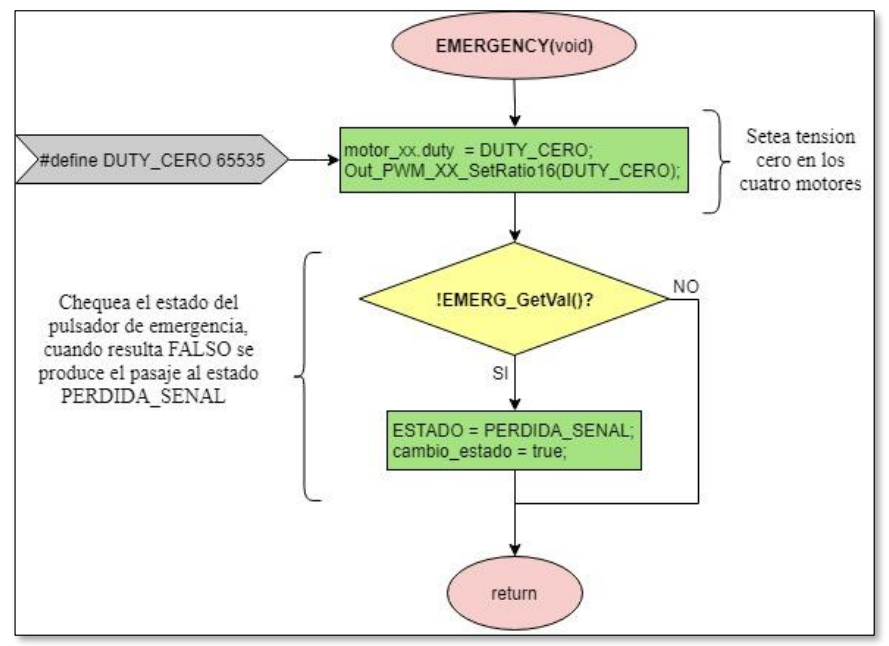
\includegraphics[width=0.8\textwidth]{diagramaFlujo.png}\par}
\end{centering}
\end{figure}


Por otro lado, a lo largo del código se utilizan estructuras condicionales (\textit{if, switch}, etc.) para determinar el flujo de ejecución. A su vez, las funciones que acceden directamente al hardware están integradas en la lógica del control (manejo del ciclo de control), lo que indica una baja separación entre la capa de abstracción del hardware y la gestion del cilo de control. Esto es acompañado con un diseño procedimental, con una serie de pasos secuenciales y un control centralizado en el flujo principal \verb|main|.

Otros inconvenientes referidos al cambio que están presentes en el código:
\begin{itemize}
\item El código parece estar compuesto por funciones largas y bloques monolíticos sin modularidad clara. Esto dificulta la localización y modificación de funcionalidades específicas, ya que los cambios pueden propagarse a otras partes del sistema que no son deseadas.
\item Los estados se definen en variables y se utilizan sentencias \textit{if} o \textit{switch} para cambiar el comportamiento de las funciones. Como se vió en la Sección \ref{cap:state} esto no es una buena práctica cuando se prepara el sistema para el cambio.
\item Hay valores ``hardcodeados'' (constantes definidas fijas en el código). Si estos valores cambian, es necesario modificar el código fuente, aumentando el riesgo de introducir errores. Además, se utilizan múltiples variables globales, las cuales añaden acoplamiento entre funciones y se debe ser cuidadoso al momento de introducir cambios que las afecten.
\item Las dependencias entre funciones están estrechamente acopladas. Lo que provoca que los cambios puedan requerir modificaciones significativas en diferentes secciones de código.
\item El manejo de errores parece ser inconsistente o inexistente en varias secciones. Es decir, no hay una decición de diseño que comtemple la existencia de posibles errores durante la ejecución. Esto puede llevar a comportamientos impredecibles y dificultar el diagnóstico de problemas.
\end{itemize}

\subsubsection*{Conclusión}

El diseño del código parece estar orientado a cumplir con un objetivo específico mediante un flujo procedimental y un control directo de los periféricos del hardware. Este enfoque es funcional, pero carece de modularidad y abstracción, lo que lo hace menos flexible y más difícil de mantener. La estructura actual no parece diseñada para escalar con nuevas funcionalidades.

\subsection*{Ejemplo}

A continuación se describirá un ejemplo extraído de \cite[Sección. 3.4]{douglass},s e explicará la solución prouesta en el mismo libro y luego se propondrá una solución orientada al cambio.

\subsubsection*{Requisitos del sistema de control de un brazo robótico}
\label{requisitos}

Se necesita desarrollar el software de control de un brazo robótico que consta de tres \gls{actuadores}, dos \glspl{pasoapaso} (uno para rotar en su base y otro para extender o retraer el brazo) y una pinza que se puede cerrar o abrir. En le Figura \ref{brazoEsquema} podemos observar un esquema del hardware. Para controlar el comportamiento del brazo, se provee una función compleja la cual toma coordenadas en el espacio y devuelve una secuencia de pasos para que el brazo tome un objeto en la posición determinada por las coordenadas. Cada paso consta de una orden para cada actuador del brazo robótico. Estos se deben ejecutar de manera secuencial, es decir que el paso número dos empezará su ejecución solo si el primero culminó completamente y con éxito. En caso de que las coordenadas sean inalcanzables la función devuelve cero pasos. Si se produce un error durante la ejecución de un paso, se detiene la ejecución del sistema.

Controlar \glspl{pasoapaso} es más complejo de lo que parece. Habitualmente, se gestionan con dos funciones: una que define el sentido de giro y otra que ordena dar un solo paso. La longitud de cada paso viene determinada por el hardware del motor. Por lo tanto, para lograr movimientos más largos, se deben ejecutar múltiples pasos, lo que requiere un control exhaustivo del software. Este es un requerimiento implicito que el sistema tiene y debemos abarcar.

\begin{figure}[h]
\caption{Esquema del brazo robótico.}
\label{brazoEsquema}
\begin{centering}
{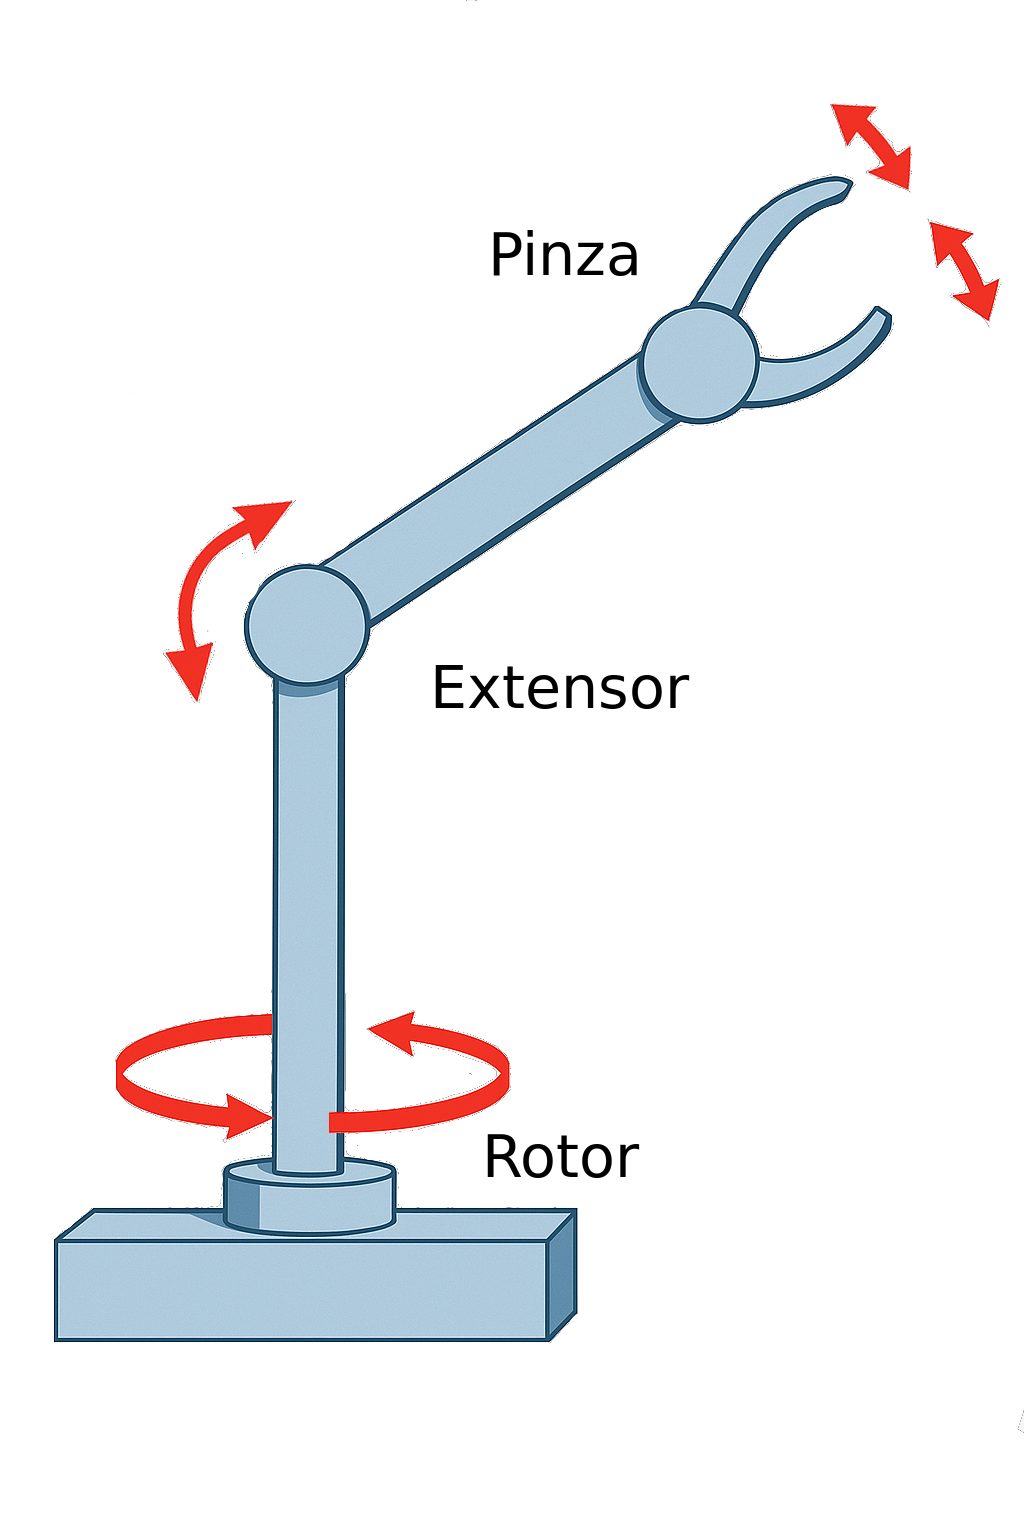
\includegraphics[width=0.5\textwidth]{brazo3.png}\par}
\end{centering}
\end{figure}

\subsubsection*{Solución propuesta en el libro de Douglass}

El ejemplo que plantea el libro es similar al descrito, pero el brazo robótico tiene más actuadores. Como solución, se propone la creación de un módulo llamado \textbf{RobotArmManager}, cuya función es gestionar los actuadores y coordinar su comportamiento. Además, para cada tipo de articulación o actuador, se crea un módulo específico encargado de su control. Este módulo proporciona métodos para consultar el estado actual (posición, longitud, etc.) y otros para establecer un valor, similar a un \textit{set-point}. Dichos métodos desempeñan el rol de ejecutores de la acción, es decir, toman un valor \textit{set-point}, ejecutan la acción y retornan \verb|True| si fue satisfactoria, o \verb|False| en caso contrario.

El comportamiento del sistema comienza con la generación de una lista de pasos a realizar. Luego, se itera sobre esta lista ejecutando las acciones definidas en cada paso. Como el sistema debe interrumpir la ejecución si encuentra un error, el \textbf{RobotArmManager} verifica el valor de retorno tras cada acción. La ejecución de un movimiento completo finaliza cuando se completan todos los pasos generados previamente por la función compleja que se mencionó en los requerimientos. En este caso es llamada \verb|graspAt(i: Coordenadas)|.

La solución propuesta parece estar un nivel de abstracción por encima de lo que se esperaría para este caso. Aunque no hay suficiente información sobre el hardware del brazo robótico, sabemos que utilizar \glspl{pasoapaso} no es tan simple como invocar un método. Este proceso suele requerir el control continuo, operando mediante pulsos que hacen que el motor avance un paso. Por lo tanto, los módulos encargados de los movimientos probablemente tengan más responsabilidades de las que se plantean en el libro. Esto va en contra de las prácticas de la \gls{IS}, que establecen que un módulo debe ocultar un solo elemento de cambio. Además, sería necesario implementar un sistema de control más complejo, utilizando algún tipo de \textit{timer} o espera, para garantizar que el \gls{pasoapaso} tenga el tiempo necesario para actuar.

De todas formas, suponiendo que los módulos mencionados se adaptan al hardware subyacente, la manera en la que el \textbf{RobotArmManager} interactúa con ellos es rígida, tanto por la invocación directa como por la dependencia del valor de retorno. Esto se evidencia en el código resultante, que incluye múltiples sentencias if consecutivas \cite[Pág. 107]{douglass}. Esta estructura provoca que, ante un cambio en el comportamiento de los módulos que interactúan con el hardware, el \textbf{RobotArmManager} pueda verse afectado, lo que requeriría una modificación en su implementación.

Por otro lado, un ítem de cambio común son las estructuras de datos, como se mencionó en la Sección \ref{listaItems}. Por ello, establecer el uso de una lista directamente en la interfaz de un módulo no responde a una buena práctica.

Es posible que el problema haya sido simplificado con fines didácticos. La forma planteada parece alejarse de una implementación realista, dejando requisitos menos específicos que podrían dar lugar a diferentes interpretaciones.

Douglass aplicar el patrón \textit{Mediator} \ref{anexoMediator} de Gamma. De manera que \textbf{RobotArmManager} cumple el rol de \textbf{Mediador} y cada módulo que se encarga de manejar cada actuador cumple el rol de \textbf{Colega}. Los autores en \cite{Gamma:1995:DPE:186897} establecen que el patrón es aplicable en los siguientes casos:
\begin{itemize}
\item Un conjunto de módulos se comunica de maneras bien definidas pero complejas. Las interdependencias resultantes son poco estructuradas y difíciles de comprender.

\item Reutilizar un módulo resulta complicado porque este se refiere y se comunica con muchos otros módulos.

\item Un comportamiento distribuido entre varios módulos debería ser personalizable sin requerir una gran cantidad de submódulos.
\end{itemize}

La estructura construida por Douglass es similar al patrón y logra el objetivo de reducir el acoplamiento, evitando que los módulos se refieran directamente entre ellos.



\subsection*{Subsistemas de control}
\label{subsistema}
\addcontentsline{toc}{subsection}{Subsistemas de control}

Para dar la solución orientada al cambio que se propone en este trabajo, primero se introducirá el concepto de lo que llamaremos \textbf{Subsistema de control}. El cual fue extraído del trabajo realizado en el robot desmalezador \citep{paperPomponio} y se utilizará como diseño de referencia.

En un sistema complejo donde se controlan múltiples propiedades físicas, el sistema se divide en subsistemas. Cada subsistema controla una propiedad específica y se organiza según el estilo arquitectónico de control de procesos \ref{arqControlProc}. De esta manera, se logra independencia entre el control de cada propiedad, lo que prepara al sistema para cambios individuales en el control de cada una de ellas. Además, se promueve la reutilización del código, ya que un subsistema de control diseñado para manejar una propiedad específica puede aplicarse en diferentes escenarios o sistemas.

Estos subsistemas de control son una estructura de módulos relacionados mediante herencia, composición o invocación. Cuyo trabajo es lograr que cierta propiedad fisica alcance el valor deseado. Para hacerlo interactua con la variable a manipular y las variables medidas relacionadas. En la Figura \ref{modulosSub} se puede observar de manera concreta los módulos que forman parte de cada componente de un subsistema. Para permitir la interacción con un cliente externo deben proveer una interfaz que permita establecer un valor al que se quiera llevar la propiedad (ver \textit{setPoint} en la Tabla \ref{tab:conceptosArq}) y que indique el comienzo de la tarea de control.

\begin{figure}[H]
\caption{Módulos de un subsistema de control y el componente al que pertenencen.}
\label{modulosSub}
\begin{center}
\begin{tikzpicture}\sf

\tikzstyle{moduloL}=[minimum width=3cm, minimum height=1.5cm,inner sep=2mm,above right,draw,align=center, font=\scshape] 

\tikzstyle{supest}=[rounded corners=1.5mm, minimum width=2cm,inner sep=2mm,draw,text width=2cm]

\tikzstyle{nombre}=[inner sep=0mm, font=\bfseries]

\tikzstyle{pipe}=[-latex,thick,line width=4pt]

\tikzstyle{nombreLogico}=[inner sep=0mm, font=\scshape, minimum width=1.5cm]

%---figura control-----
\tikzstyle{ctrl}=[shape=circle,draw,minimum width=2.5cm,text width=2cm, inner sep=2, align=center,font=\scshape];


%----figura de sensor---
\tikzstyle{sensor}=[draw,circle, minimum width=1cm,after node path={(\tikzlastnode) circle (0.2cm)}]
% se usa así: \draw node[sensor]{};

%---------------------------------------
%---control del proceso rueda----
\node[ctrl, text width=1.8cm] (0,0) (controlR){Control};
%
\node[moduloL, below=2cm of controlR, minimum width=3cm](procesoArq){Proceso};
%%
\draw node[sensor, below=2cm of procesoArq](sensorCte){};
%%
%%%puntos para hacer las flechas de las señales hacia los sensores
\node[below=4.5cm of procesoArq](pto2){};
%%
\draw[dashed, -latex](procesoArq)--(pto2);
%%
\node[nombreLogico, below left=-0.1cm and 0.1cm of sensorCte, text width=1.5cm]{Sensor};
%%
%%%---pipes
\draw[pipe] (sensorCte.west) -| (-2.3,-4) |- (controlR.west);

%
%%
\path let \p1 = (controlR) in
  \draw[-latex](\x1-4,\y1+1) -- node[at start, yshift=10pt, xshift=15pt]{\normalsize set point}(controlR.125);
  
\path let \p1 = (controlR) in
  \draw[*-latex](\x1-4,\y1+0) -- node[at start, yshift=10pt, xshift=15pt]{\normalsize evento}(controlR.165);
 
%\draw[-latex](controlR) -- node[midway, right] (procesoArq);
\draw[-latex] (controlR) -- (procesoArq);


%%
\node[below left=0.7cm and -0.7cm of controlR, text width=1.3cm]{};
\node[below right=0.7cm and -0.5cm of controlR, text width=1.3cm]{};
%%
%

\draw[dash pattern=on 6pt off 2pt on 2pt off 2pt] (-3, -2.4) -- (13, -2.4);
\draw[dash pattern=on 6pt off 2pt on 2pt off 2pt] (-3, -5.7) -- (13, -5.7);
\draw[dash pattern=on 6pt off 2pt on 2pt off 2pt] (2, 3) -- (2, -10);




\umlclass[right=1.25cm of controlR]{Control}
{}
{setPoint(i: Measure)\\
control() \\
connectionRead() \\
setAlgoritmo(i: Algoritmo) \\
setConnection(i: Pipe)
}

\umlclass[right=2cm of sensorCte]{Sensor}
{}
{setConnection(i: Pipe) \\
signal()
}
\umlnote[below=1cm of Sensor,width=4cm]{Sensor}{
signal()\{ \\
\ \ \ \ value = getValue()\\
\ \ \ \ pipe.write(value)\\
\}
}


\umlclass[right=1cm of procesoArq]{Pipe}
{}
{read(): Measure \\
write(i: Measure)
}

\umlclass[right=3cm of Pipe]{Actuador}
{}
{actuar()
}


\umlnote[below=1.5cm of Actuador, width=5cm]{Actuador}{
Por lo general se desacopla usando el patrón \textit{command} y su uso puede ser más complejo que solo ejecutar una función.
}



\umlclass[right=1.5cm of Control]{Algoritmo}
{}
{calcular(): Measure
}

\umluniaggreg[]{Control}{Algoritmo}

\end{tikzpicture}
\end{center}
\end{figure}

Los módulos principales son los siguientes:

\declareCMod{Control}
\declareCMod{Algoritmo}
\declareCMod{Pipe}
\declareCMod{Actuador}
\declareCMod{Sensor}


\begin{itemize}
\item \Control: encargado de proveer una interfaz a clientes desde la cual se realizan todas las tareas referidas al control.
\item \Actuador: encapsula el dispositivo de hardware que manipula la variable física.
\item \Sensor: encapsula el dispositivo de hardware utilizado para recibir información del mundo físico, pueden existir múltiples sensores.
\item \Pipe: módulo que se ubica entre \Control y los sensores tiene un funcionamiento sencillo, ofrece dos métodos: uno para escribir y otro para leer. De esta manera, un módulo escribe y otro lee, lo que permite comunicación entre ellos sin necesidad de invocación directa. Encapsula la comunicación entre módulos.
\end{itemize}

Una vez decidido el valor deseado o \textit{set-point} al cual se busca aproximar la variable física, se puede comenzar a ejecutar el ciclo de control. Este será invocado de manera periódica mediante un temporizador. Siguiendo el estilo arquitectónico de control de procesos, se define que un ciclo de control consta de los pasos mostrados en el Código \ref{usoSubsistema}. En primer lugar, se establece el set-point utilizando el método \verb|setPoint(i: Measure)| de \Control. Luego, se indica a \Sensor que escriba en \Pipe el valor de la variable medida. En la línea 3, se solicita a \Control que lea dicho valor y, una vez recuperado, pueda decidir qué cambios aplicar en \Actuador. De esta manera, luego de una serie de iteraciones se espera que la variable física se encuentre más cerca del \textit{set-point}.

\begin{lstlisting}[caption=Ejemplo de uso del subsistema.,label={usoSubsistema}]
control.setPoint(valorDeseado)
sensor.signal()
control.connectionRead()
control.control()
\end{lstlisting}

Notar que en la Figura \ref{modulosSub} aparece un módulo que no fue mencionado anteriormente, \Algoritmo el cual se encarga de los cálculos necesarios para determinar de qué manera accionar sobre el o los actuadores. \Control delega en \Algoritmo la tarea de realizar los computos. Si el algoritmo cambia (recordar que es un item de cambio probable \ref{listaItems}) solo ese módulo se ve afectado. Si se definió correctamente la interfaz, solo se agrega otro módulo con el nuevo algoritmo. No es necesario modificar el módulo \Control.

En el ámbito de la robótica se aplican diferentes técnicas de estabilización\footnote{La estabilización es crucial para evitar oscilaciones, reducir el tiempo de respuesta y minimizar sobrepasos, garantizando un control preciso y eficiente. Un sistema bien ajustado responde de manera estable ante perturbaciones externas y optimiza el consumo energético, mejorando la fiabilidad y el desempeño en aplicaciones como robótica y automatización.} de variables físicas, las cuales permiten alcanzar un cierto \textit{set-point} y mantenerse en el, por ejemplo, los controladores \gls{PID}\cite{pidlibro} (controlador proporcional, integral y derivativo). Este tipo de técnicas puede ser usada siguiendo la estructura módular propuesta y, en particular, los cálculos asociados se definirían en este módulo \Algoritmo.

\declareCMod{ControlSeguimiento}

Como se mencionó previamente, cuando se presentó el ejemplo extraído de \citep{douglass}, los \glspl{pasoapaso} requieren de un seguimiento en tiempo real para cumplir su cometido. Por ejemplo, suponga que \Control decidió que es necesario que el motor gire 30\degree, y que un paso del motor representa solo 5\degree. En ese caso, deberíamos aplicar múltiples cambios en el actuador (motor) para alcanzar el objetivo. Además, si el motor requiere menos tiempo que el intervalo entre ciclos de control para completar un paso, estaríamos desperdiciando una parte significativa de tiempo. Es por esto que se presenta una modificación del módulo \Control para manejar actuadores que necesitan un seguimiento entre ciclos de control. A este módulo modificado lo llamaremos \ControlSeguimiento.

Por un lado, se agrega una nueva interrupción periódica que invocará al método \verb|cicle| del módulo \ControlSeguimiento cada determinado tiempo. El periodo es menor al del ciclo de control y puede variar en base al actuador que se utilice.
Además, es necesario dotar al módulo de un estado. De modo que existan dos estados básicos, en espera, cuando no se está realizando un ciclo de control y trabajando, cuando se haya establecido un \textit{set-point} y se esté activamente trabajando para llegar a él. Para hacerlo se hace uso de un nuevo método y del patrón \textit{state}\footnote{El uso de este patrón está explicada en la Sección \nameref{cap:state}.}. La estructura de módulos obtenida de aplicar el patron y extender \Control se puede observar en la Figura \ref{controlState}.

\begin{figure}[H]
\caption{Estructura módulo \ControlSeguimiento.}
\label{controlState}
\begin{center}
\begin{tikzpicture}\sf
\umlclass[x=-4]{ControlSeguimiento}
{}
{setPoint()\\
control() \\
cicle() \\
connectionRead() \\
setAlgoritmo(i: Algoritmo) \\
changeState(i: State)
}
\umlnote[above right=1cm and -4cm of ControlSeguimiento, width=4cm]{ControlSeguimiento}{
control()\{\\
\ \ \ \ return st.control(this) \\
\}\\
cicle()\{\\
\ \ \ \ return st.cicle(this) \\
\}\\
}

\umlclass[x=4, y=3,type=abstract]{State}
{}
{
\umlvirt{control(i: Control)} \\
\umlvirt{cicle(i: Control)} \\
}

\umlclass[x=2,y=-2]{Waiting}
{}
{
control(i: Control) \\
cicle(i: Control) \\
}


\umlclass[x=6,y=-2]{Working}
{}
{
control(i: Control) \\
cicle(i: Control) \\
}

\umlnote[below left=1cm and -4cm of ControlSeguimiento, width=4cm]{ControlSeguimiento}{
control cada 100 ms\\
cicle cada 1.5 ms\\
}

\umlnote[below left=1cm and -3cm of Waiting, width=5cm]{Waiting}{
control(Control c)\{\\
\ \ \ \ controlar... \\
\ \ \ \ c.changeState(working)\\
\}\\
cicle()\{\\
\ \ \ \ return \\
\}\\
}
}

\umlnote[below left=1cm and -5cm of Working, width=5cm]{Working}{
control(Control c)\{\\
\ \ \ \ return \\
\}\\
cicle()\{\\
\ \ \ \ controlar... \\
\ \ \ \ si se llegó al setpoint \{\\
\ \ \ \ \ \ \ \ c.changeState(waiting)\\
\ \ \ \ \}\\
\}\\
}
}


\umlinherit[geometry=|-|]{Waiting}{State}
\umlinherit[geometry=|-|]{Working}{State}
\umluniaggreg[geometry=-|-,arg1=st, pos1=0.5]{ControlSeguimiento}{State}

\end{tikzpicture}
\end{center}
\end{figure}

\declareCMod{Waiting}

En consecuencia, cuando se ejecuta un ciclo de control y se determina la necesidad de aplicar un cambio en los actuadores controlados por \ControlSeguimiento, su estado interno cambiará. De este modo, comenzará a atender la interrupción periódica de menor periodo. Al ejecutarse esta interrupción, se verificará nuevamente si se ha alcanzado el \textit{set-point}. De ser así, el sistema transicionará al estado de espera \Waiting, donde se ignorará la interrupción de menor período, pero se continuará atendiendo la interrupción que marca el inicio del ciclo de control. En caso contrario, aplicará el cambio en el actuador sin transcicionar, con el fin de que en una invocación futura la variable física se encuentre cerca del valor esperado. La estructura presnetada permite un seguimiento preciso en la aplicación de cambios a los actuadores que lo requieran, como los \glspl{pasoapaso}.

La documentación de la aplicación del patrón \textit{State} en este caso esta presente en la Figura \ref{docStateControl}.

\begin{figure}
\caption{Documentacion de la aplicación del patrón State en el módulo Control.}
\label{docStateControl}
\begin{pattern}[]{Estados de operación del controlador}{Algorithm}{idFigAlg}
\based{Estado (State)}
\why{\textbf{Cambios previstos}: El controlador lleva a cabo el control dependiendo del estado en el que se encuentre. Podrían cambiar el comportamiento requerido de algunos de los estados definidos o bien podría ser necesario agregar nuevos estados con sus correspondientes comportamientos.

\textbf{Funcionalidad}: Dependiendo del estado, los métodos control y cicle deben comportarse de manera diferente. A su vez, pueden cambiar de manera dinámica. En caso de que no se esté realizando una acción sobre alguno de los actuadores que 
}
\assigns
\is{ControlSeguimiento}{Contexto}
\is{State}{Estado}
\is{Waiting}{EstadoConcreto}
\is{Working}{EstadoConcreto}
\end{pattern}
\end{figure}


Por último, repasemos los beneficios de utilizar subsistemas de control. Este diseño permite el control de una variable específica del proceso, como la velocidad de giro de una rueda o la posición de un \gls{pasoapaso}. Si se requiere controlar otra propiedad de forma independiente, se hará con otro subsistema. El enfoque principal es encapsular el control de cada propiedad de manera individual. Esto permite que cada una pueda cambiar de forma aislada sin afectar al resto del sistema. Además, facilita la extensibilidad, ya que añadir nuevas propiedades físicas con sus respectivos actuadores y sensores solo requiere la creación de nuevos módulos. Este diseño proporciona una capa de abstracción que permite construir sobre los subsistemas un controlador general, el cual se encarga de involucrar y sincronizar a cada uno para llevar a cabo comportamientos más complejos.



\subsubsection*{Solución orientada al cambio}

Esta solución se basa en aquella dada al problema del robot desmalezador en \citep{paperPomponio}, pero aplicada al brazo robotico descripto en \ref{requisitos}. Por lo tanto, se aplica el concepto de subsistemas que se introdujo previamente. Para ello primero se debe identificar las propiedades del mundo físico a controlar. Lo que se requiere es modificar la posición y el estado (abierto o cerrado) de la pinza del brazo. Para hacerlo se cuenta con distintos actuadores que intervienen diferentes propiedades físicas. En particular dos \gls{pasoapaso} y la pinza. Además, en los requisitos se especifica que se cuenta con una función que genera una lista de pasos con ordenes para cada actuador. De esta manera se define un subsistema de control por cada actuador que serán los encargados de llevar a cabo las ordenes generadas. Un ejemplo de orden es rotar brazo a 30\textdegree, esta hace referencia a actuar sobre el \gls{pasoapaso} de la base del brazo. En particular, estableciendo un \textit{set-point} de posición igual a 30\textdegree. 

\declareCMod{MainController}

Para coordinar los subsistemas se propone un controlador principal llamado \MainController, el cual provee el método \verb|graspAt(i: Coordenadas)| al cliente, realiza la generación de los pasos y controla su ejecución. La estructura es como la que se describe en la Figura \ref{diagramaRobotico}.


\begin{figure}[H]
\caption{Diagrama de los componentes del sistema brazo robótico.}
\label{diagramaRobotico}
\begin{center}

\begin{tikzpicture}\sf


\umlsimpleclass{MainController}
\umlsimpleclass[left=2cm of MainController]{Cliente}

\umlsimpleclass[below left=3cm and 2cm of MainController]{RotorCtrl}
\umlsimpleclass[below=0.5cm of RotorCtrl]{PipeR}
\umlsimpleclass[below=0.5cm of PipeR]{Rotor}
\umlsimpleclass[below=0.5cm of Rotor]{SensorPosRotor}

\umlsimpleclass[below=3cm of MainController]{PinzaCtrl}
\umlsimpleclass[below=0.5cm of PinzaCtrl]{PipeP}
\umlsimpleclass[below=0.5cm of PipeP]{Pinza}
\umlsimpleclass[below=0.5cm of Pinza]{SensorPosPinza}

\umlsimpleclass[below right=3cm and 2cm of MainController]{ExtensorCtrl}
\umlsimpleclass[below=0.5cm of ExtensorCtrl]{PipeE}
\umlsimpleclass[below=0.5cm of PipeE]{Extensor}
\umlsimpleclass[below=0.5cm of Extensor]{SensorPosExtensor}



\node[draw, rounded corners, inner sep=10pt, fit=(RotorCtrl) (PipeR) (Rotor) (SensorPosRotor)] (RotorGroup) {};
\node[above=0pt of RotorGroup.north, xshift=-1cm] {Subsistema Rotor};

\node[draw, rounded corners, inner sep=10pt, fit=(PinzaCtrl) (PipeP) (Pinza) (SensorPosPinza)] (PinzaGroup) {};
\node[above=0pt of PinzaGroup.north, xshift=-0.5cm] {Subsistema Pinza};

\node[draw, rounded corners, inner sep=10pt, fit=(ExtensorCtrl) (PipeE) (Extensor) (SensorPosExtensor)] (ExtensorGroup) {};
\node[above=0pt of ExtensorGroup.north, xshift=1cm] {Subsistema Extensor};


\umluniassoc{Cliente}{MainController}
\umluniassoc{MainController}{RotorCtrl}
\umluniassoc{MainController}{PinzaCtrl}
\umluniassoc{MainController}{ExtensorCtrl}
\umluniassoc{RotorCtrl}{MainController}
\umluniassoc{PinzaCtrl}{MainController}
\umluniassoc{ExtensorCtrl}{MainController}

\end{tikzpicture}

\end{center}
\end{figure}

\declareCMod{Mediator}
\declareCMod{College}

Se puede pensar que el gráfico guarda cierta similitud conceptual con el patrón \textit{mediator} \ref{anexoMediator}. Este patrón encapsula cómo interactúan los módulos entre sí, con el fin de permitir variar su interacción de manera independiente. Un módulo \Mediator coordina el trabajo de los \College, en este caso los subsistemas. Gamma, en \cite{Gamma:1995:DPE:186897}, indica que el patrón puede aplicarse cuando se tiene un conjunto de módulos que se comunican de manera compleja pero fija. En este caso, la comunicación no es demaciado compleja, pero sí lo suficiente como para justificar el uso del patrón. En particular, el \MainController establece los \textit{set-points} de cada subsistema y desencadena el proceso de control en cada uno. A la inversa, los subsistemas informan cuándo alcanzan el \textit{set-point} o cuándo encuentran un error. A su vez, los subsistemas no se comunican directamente entre sí: toda la interacción pasa por el \MainController. Esto permite, por ejemplo, que la pinza pueda cerrarse únicamente cuando el brazo esté extendido, sin necesidad de que los módulos se comuniquen entre sí. Tradicionalmente, el módulo encargado de manejar el rotor le avisaría al módulo encargado de controlar la pinza que finalizó su tarea. Esto, sin embargo, genera un acoplamiento entre módulos, problema que ya se comentó previamente en esta tesina. En cambio, con este patrón, \RotorCtrl no sabe ni tiene noción de la existencia de \PinzaCtrl o \ExtensorCtrl. Toda la comunicación pasa a través de \MainController, lo que desacopla los módulos controladores.

Ahora, se detallarán los módulos que conforman cada componente comenzando por los módulos básicos que debemos crear para representar el hardware dado. Los módulos de la Figura \ref{estructuraActuadores} representan \glspl{pasoapaso}\footnote{Se utiliza el mismo diseño propuesto para el robot desmalezador\cite{paperPomponio}.}, los cuales para ser controlados se deben primero hablitar el dispositivo utilizando \verb|enable| y configurar su dirección invocando a los métodos \verb|right| o \verb|left| para luego avanzar un paso llamando al método \verb|pulse|. Claramente para que lleguen a la posición deseada puede ser necesario invocar reiteradas veces al método \verb|pulse|. Esto será importante a la hora de diseñar el subsistema que controlará cada dispositivo.

En cambio, en el caso de la pinza (ver Figura \ref{moduloPinza}) se utiliza un dispositivo que tiene dos estados, abierto o cerrado, por lo que solo se tienen dos métodos para abrir o cerrar la pinza.

\begin{figure}[H]
\caption{Actuadores paso a paso.}
\label{estructuraActuadores}
\begin{center}
\begin{tikzpicture}\sf
\umlclass[type=abstract]{StepDevice}
{}
{
\umlvirt{right()} \\
\umlvirt{left()} \\
\umlvirt{disable()}\\
\umlvirt{enable()} \\
\umlvirt{pulse()}
}

\umlclass[below left=2cm and -0.3cm of StepDevice]{Rotor}
{}
{
...\\
}

\umlclass[below right=2cm and -0.3cm of StepDevice]{Extensor}
{}
{
...\\
}

\umlinherit[geometry=|-|]{Rotor}{StepDevice}
\umlinherit[geometry=|-|]{Extensor}{StepDevice}

\end{tikzpicture}
\end{center}
\end{figure}


\begin{figure}[h!]
\caption{Interfaz módulo Pinza.}
\label{moduloPinza}
\begin{center}
\begin{tikzpicture}\sf
\umlclass[]{Pinza}
{}
{
abrir() \\
cerrar()
}

\end{tikzpicture}
\end{center}
\end{figure}

En la Figura \ref{sensores} se encuentran definidos los sensores asociados a cada actuador, estos heredan del módulo sensor pasivo el cual provee dos métodos, \verb|setConnection(i: Pipe)| el cual configura el \Pipe por el cual se enviará la información obtenida del sensor cuando el otra método, \verb|signal()| sea invocada.

\begin{figure}[h]
\caption{Sensores del brazo robótico.}
\label{sensores}
\begin{center}
\begin{tikzpicture}\sf
\umlclass[type=abstract]{PasiveSensor}
{}
{
\umlvirt{setConnection(i: Pipe)} \\
\umlvirt{signal()} \\
}

\umlclass[x=-5,y=-4]{SensorEstadoPinza}
{}
{
setConnection(i: Pipe) \\
signal() \\
}

\umlclass[x=0,y=-4]{SensorPosRotor}
{}
{
setConnection(i: Pipe) \\
signal() \\
}

\umlclass[x=5,y=-4]{SensorPosExtensor}
{}
{
setConnection(i: Pipe) \\
signal() \\
}

\umlnote[above left=1cm and -4cm of SensorEstadoPinza,width=5cm]{SensorEstadoPinza}{
signal()\{\\
\ \ \ \ leer estado pinza \\
\ \ \ \ pipe.write(estadoPinza)\\
\}
}

\umlinherit[geometry=|-|]{SensorEstadoPinza}{PasiveSensor}
\umlinherit[geometry=--]{SensorPosRotor}{PasiveSensor}
\umlinherit[geometry=|-|]{SensorPosExtensor}{PasiveSensor}


\end{tikzpicture}
\end{center}
\end{figure}
\declarCMod{RotorCtrl}

Para completar los módulos que conforman un subsistema de control, falta mostrar cómo se define el módulo encargado de llevar el control de cada uno. En la Sección \ref{subsistema} mencionamos dos tipos de controladores: uno básico y otro más complejo, utilizado cuando los actuadores involucrados en ese subsistema requieren un control exhaustivo, como los \glspl{pasoapaso}. En este ejemplo contamos con dos motores paso a paso: uno en el rotor de la base y otro en el extensor. Además, tenemos la pinza, que no necesita un seguimiento exhaustivo para su operación; simplemente se le indica la posición a adoptar y el hardware se encarga de ejecutarla. A continuación, mostraremos primero el módulo controlador que utilizaremos en el subsistema encargado del rotor \RotorCtrl, siendo el del extensor de estructura similar.

\declarCMod{Timer}

Como tambien fue mencionado en la Sección \ref{subsistema}, es necesario añadir una interrupcion con un periodo menor al del ciclo de control y que está definido por el hardware a controlar. Por ejemplo, para el control del motor paso a paso que maneja la direccion del robot desmalezador en \cite{paperPomponio} se eligió 1.5\textit{ms}. Esta interrupcion es lanzada por un dispositivo de hardware externo que actua como temporizador. El módulo que encapsula su comportamiento es \Timer y tiene la estructura mostrada en la Figura \ref{moduloTimer}.

\begin{figure}[H]
\caption{Módulo Timer}
\label{moduloTimer}
\begin{center}
\begin{tikzpicture}\sf
\umlclass[]{Timer}
{}
{
setPeriod(i: Real) \\
start() \\
stop() \\
tickHandler()
}

\umlnote[above right=-2cm and 1cm of Timer,width=7cm]{Timer}{
tickHandler() \{ \\
cmdRotorCicle.execute() \\
\}
}

\umlsimpleclass[below right=-1cm and 3cm of Timer]{Command}
\umluniassoc[arg1=cmdRotorCicle,pos1=0.5, anchor1=-32]{Timer}{Command}
\end{tikzpicture}
\end{center}
\end{figure}

El método \verb|tickHandler()| ejecutará comandos siguiendo el patrón \textit{Command} \ref{anexoCommand} por cada subsistema que lo necesite. En particular, el comando es utilizada para desacoplar el \Timer del módulo que controla el subsistema. Este uso del patrón fue explicado en la Sección \ref{patronCommand}. En la Figura \ref{docCommandTimer} se puede observar la documentación de la aplicación del patrón \textit{Command} para este caso.

\begin{figure}[H]
\caption{Documentación de la aplicación del patrón \textit{Command} para el desacople de ejecuciones que invoca el Timer.}
\label{docCommandTimer}
\begin{pattern}[]{Comando para manejar interrupciones generadas por el Timer.
Sustitución de callback}{Algorithm}{idFigAlg}
\based{Orden (Command)}
\why{\textbf{Cambios previstos}: Las acciones a llevar a cabo ante una interrupcion provocada por el Timer podrían cambiar; o incluso podría cambiar el receptor de dichas acciones, que actualmente es Controller.

\textbf{Funcionalidad}: Se mantienen los niveles de abstracción. El módulo Timer, desconoce la existencia de módulos de niveles superiores como el Controller.
}
\assigns
\is{Command}{OrdenConcreta}
\is{Timer}{Invocador}
\is{Controller}{Receptor}
\end{pattern}
\end{figure}


Una vez solucionada la invocación, introduciremos un nuevo módulo que será utilizado en \RotorCtrl. Como vimos en la Sección \ref{subsistema}, es necesario agregar un estado al controlador; para ello hacemos uso del patrón \textit{State}. Este estado define los modos de operación de \RotorCtrl: uno para atender el ciclo de control y otro para atender la interrupción de menor período, que utilizamos para dar seguimiento a la aplicación del cambio en el motor paso a paso. Para implementarlo, construimos los módulos mostrados en la Figura \ref{operationState}.

\begin{figure}[H]
\caption{Módulos que forman parte del patrón \textit{State} que son necesarios para complementar al módulo RotorCtrl.}
\label{operationState}
\begin{center}
\begin{tikzpicture}\sf
\umlclass[type=abstract]{OperationState}
{}
{
\umlvirt{control(i: RotorCtrl)} \\
\umlvirt{move(i: RotorCtrl)} \\
}

\umlclass[x=-3,y=-4]{Moving}
{}
{
control(i: RotorCtrl) \\
move(i: RotorCtrl) \\
}

\umlclass[x=3,y=-4]{Waiting}
{}
{
control(i: RotorCtrl) \\
move(i: RotorCtrl) \\
}

\umlinherit[geometry=|-|]{Moving}{OperationState}
\umlinherit[geometry=|-|]{Waiting}{OperationState}

\umlnote[above left=1.5cm and -1.5cm of Moving,width=5cm]{Moving}{
control(RotorCtrl c)\{\\
\ \ \ \ return\\
\}\\
move(RotorCtrl c)\{\\
\ \ \ \ if se llego al setpoint \{\\
\ \ \ \ c.changeOpState(waiting)\\
\ \ \ \ \}else\{\\
\ \ \ \ ... dar un paso ...\\
\ \ \ \ \}\\
\}
}

\umlnote[above right=1.5cm and -1.5cm of Waiting,width=4cm]{Waiting}{
control(RotorCtrl c)\{\\
...\\

\}\\
move(RotorCtrl c)\{\\
\ \ \ \ return\\
\}
}

\end{tikzpicture}
\end{center}
\end{figure}
\declareCMod{Algoritmo}

Siguiendo con la propuesta de creación de subsistemas, también se define el módulo \Algoritmo que encapsula los cálculos necesarios para determinar cómo accionar sobre los actuadores. Su interfaz se puede observar en la Figura \ref{complementariosController}.

\begin{figure}[H]
\caption{Módulos complementarios a Controller.}
\label{complementariosController}
\begin{center}
\begin{tikzpicture}\sf
\umlclass[x=3]{Algoritmo}
{}
{
compute(i: Data): Measure
}

\end{tikzpicture}
\end{center}
\end{figure}

Con todos los módulos necesarios ya definidos, veamos ahora en la Figura \ref{estructuraController} el diagrama de \{RotorCtrl}.

\begin{figure}[H]
\caption{Diagrama del módulo RotorCtrl}
\label{estructuraController}
\begin{center}
\begin{tikzpicture}\sf
\umlclass[]{RotorCtrl}
{}
{
setConnection(i: Pipe) \\
readConnection() \\
setSetPoint(i: Measure) \\
getAlgoritmo(): Algoritmo \\
changeOpState(i: OperationState) \\
move() \\
control()
}

\umlsimpleclass[above right=-2.5cm and 2cm of RotorCtrl]{Algoritmo}
\umlsimpleclass[above right=-3.5cm and 2cm of RotorCtrl]{OperationState}
\umlsimpleclass[above right=-4.5cm and 2cm of RotorCtrl]{Pipe}

\umluniaggreg[anchor1=6]{RotorCtrl}{Algoritmo}
\umluniaggreg[anchor1=-12,arg1=st,pos1=0.3]{RotorCtrl}{OperationState}
\umluniaggreg[anchor1=-29]{RotorCtrl}{Pipe}

\umlnote[below left=1cm and -2cm of RotorCtrl]{RotorCtrl}{
move()\{\\
\ \ \ \ st.move(this)\\
\}
}

\umlnote[above=1cm of Algoritmo]{Algoritmo}{
Patrón Strategy
}

\umlnote[below right=1.5cm and -2cm of OperationState,anchor2=-20]{OperationState}{
Patrón State
}
\end{tikzpicture}
\end{center}
\end{figure}

Suponga que un cliente desea utilizar este subsistema que controla el rotor, ¿qué métodos debe ejecutar si este ya se encuentra inicializado?
En primer lugar, debe indicarle al sensor de posición que escriba el valor de lectura en \Pipe. Para ello, se ejecuta el método \verb|signal| del módulo \SensorPosRotor. A continuación, \RotorCtrl debe leer esta información desde \Pipe y almacenarla; para esto se utiliza el método \verb|readConnection|. Luego, se establece el \textit{set-point} deseado y, finalmente, se invoca el método \verb|control|, el cual delega su funcionamiento al \verb|control| de su estado interno. Si el estado actual es \Waiting, el método \verb|control| tomará los valores actuales junto con el \textit{set-point} y decidirá, utilizando el módulo \Algoritmo, qué cambios aplicar en los actuadores, en este caso sobre \Rotor. Dado que agregar todo el código para manejar un \gls{pasoapaso} puede requerir la ejecución de múltiples métodos, se puede construir un módulo que implemente el patrón \textit{Command} \ref{anexoCommand}, encapsulando qué métodos deben invocarse. Este comando permitirá tanto cambiar la dirección de giro como avanzar un paso mediante la ejecución de \verb|pulse()|. Como el motor puede girar en ambos sentidos, es posible definir dos comandos: uno para cada dirección (\CmdRotorLeft y \CmdRotorRight). Un ejemplo del método \verb|control()| para el caso del subsistema del rotor en el estado de operación \Waiting se muestra en el Código \ref{impControl} (recordando que el \textit{set-point} del subsistema del rotor corresponde a una medida en grados).

\begin{lstlisting}[caption=Ejemplo de implementación del método control del módulo Waiting.,label={impControl}]
control(Controller controller) {
    setPoint = data.getSetPoint()
    current = data.getCurrent()
    dif = controller.algoritmo.calculate()
    if abs(dif) > LIMIT_ACCEPT and dif > 0 {
        cmdRotorLeft.execute()
    }
    if abs(dif) > LIMIT_ACCEPT and dif < 0 {
        cmdRotorRight.execute()        
    }
    controller.changeOperationState(moving)
    return
}
\end{lstlisting}

El método \verb|move| tendrá un comportamiento similar pero en el caso de cambiar de estado lo hará a \Waiting.

Con la presentación del módulo \RobotCtrl finalizamos la definición del subsistema rotor. Además de este, deben crearse los módulos correspondientes al subsistema extensor, el cual resulta similar al del rotor.
Por último, se debe definir el subsistema pinza, que es más simple que los anteriores, ya que no requiere de un seguimiento entre ejecuciones del ciclo de control. En consecuencia, puede emplear el controlador básico presentado en la Sección \ref{subsistema}, sin necesidad de incorporar estados, nuevas interrupciones ni el método \verb|move|.
\declareCMod{MainController}

Ya definidos los subsistemas, podemos continuar con la construcción de los módulos que conforman la Figura \ref{diagramaRobotico}. En este punto, resta abordar el módulo \MainController, encargado de proveer una interfaz al cliente y, al mismo tiempo, coordinar el funcionamiento de cada subsistema. Recordando los requerimientos, sabemos que debe existir una función capaz de generar una secuencia de pasos, donde cada paso implique una acción sobre los tres actuadores. ¿Cómo diseñar este comportamiento? Una alternativa consiste en utilizar un iterador siguiendo el patrón \textit{Iterator} \ref{patronIterator} para recorrer los pasos generados por la función, y combinarlo con el patrón \textit{Command} \ref{anexoCommand} para la ejecución de cada uno de ellos. En particular, se adopta una de las variantes mencionadas por Gamma \cite{Gamma:1995:DPE:186897}, en la cual la ejecución de un comando desencadena automáticamente la ejecución de los siguientes, permitiendo encadenar acciones de manera ordenada y desacoplada.

\declareCMod{Steps}
\declareCMod{OrdenRotor}
Para esto, debemos definir el iterador, al que llamaremos \Steps, cuya interfaz se muestra en la Figura \ref{iterator}. Su correspondiente documentación se encuentra en la Figura \ref{docIterator}. En la Figura \ref{orden} se observa la estructura de módulos resultante de aplicar el patrón \textit{Command} en su variante. Además, en la Figura \ref{docCommandSteps} se presenta la documentación asociada, y en la Figura \ref{ejemploOrdenRotor} se incluye un ejemplo de una posible implementación del módulo \OrdenRotor.

\begin{figure}[H]
\caption{Interfaz módulo Steps.}
\label{iterator}
\begin{center}
\begin{tikzpicture}\sf
\umlclass[]{Steps}
{}
{
primero() \\
siguiente()\\
elementoActual(): Orden\\
haTerminado(): Bool\\
}


\end{tikzpicture}
\end{center}
\end{figure}
\begin{figure}
\caption{Documentación de aplicación del patrón \textit{Iterator}.}
\label{docIterator}
\begin{pattern}[]{Ordenes a ejecutar para realizar el movimiento requerido.}{Algorithm}{idFigAlg}
\based{Iterador (Iterator)}
\why{\textbf{Cambios previstos}: Se pueden agregar, quitar o modificar ordenes pero siempre con la posibilidad de iterar. Además, puede cambiar la estructura de datos subyacente.

\textbf{Funcionalidad}: Se logra recorrer todas las ordenes de manera secuencial.
}
\assigns
\is{Steps}{IteradorConcreto}
\is{MainControler}{AgregadorConcreto}

\end{pattern}
\end{figure}

\begin{figure}[H]
\caption{Interfaces de las ordenes de ejecución para cada subsistema.}
\label{orden}
\begin{center}
\scalebox{.75}{
\begin{tikzpicture}\sf

\umlclass[type=abstract]{Orden}
{}
{
\umlvirt{ejecutar()}
}

\umlclass[below left=2cm and 4.5cm of Orden]{OrdenRotor}
{
OrdenRotor(i: Measure)
}
{
ejecutar()
}

\umlclass[below left=2cm and -1cm of Orden]{OrdenExtensor}
{
OrdenExtensor(i: Measure)
}
{
ejecutar()
}

\umlclass[below right=2cm and -1cm of Orden]{OrdenPinza}
{
OrdenPinza(i: Measure)
}
{
ejecutar()
}

\umlclass[below right=2cm and 4cm of Orden]{OrdenMultiple}
{
OrdenMultiple(i: OrdenRotor, \\ i: OrdenExtensor, \\i: OrdenPinza)

}
{
ejecutar()
}
\umlinherit[geometry=|-|]{OrdenRotor}{Orden}
\umlinherit[geometry=|-|]{OrdenExtensor}{Orden}
\umlinherit[geometry=|-|]{OrdenPinza}{Orden}
\umlinherit[geometry=|-|,arm1=2.54cm]{OrdenMultiple}{Orden}
\umluniaggreg[geometry=-|-, anchor1=east, arm1=1cm]{OrdenMultiple}{Orden}
\umlnote[above=4cm of OrdenMultiple,width=5cm]{OrdenMultiple}{
ejecutar() \{  \\
\ \ \ \ ordenRotor.ejecutar() \\
\ \ \ \ ordenExtensor.ejecutar() \\
\ \ \ \ ordenPinza.ejecutar() \\
\}
}

\end{tikzpicture}}
\end{center}
\end{figure}

\begin{figure}
\begin{lstlisting}[caption=Ejemplo de implementación del módulo OrdenRotor,label={ejemploOrdenRotor}]
ejecutar {
    rotorController.setSetPoint(setPoint)
    rotorSensor.signal()
    rotorController.readConnection()
    rotorController.control()
}
\end{lstlisting}
\end{figure}


\begin{figure}[h]
\caption{Documentación de la aplicación del patrón Command para el desacople de ordenes a ejecutar en cada actuador del brazo en un paso.}
\label{docCommandSteps}
\begin{pattern}[]{Comando para manejar las acciones que deben ser ejecutadas en un paso en cada actuador.}{Algorithm}{idFigAlg}
\based{Orden (Command)}
\why{\textbf{Cambios previstos}: Las acciones a llevar a cabo para cada actuador pueden cambiar, se pueden agregar o quitar actuadores.

\textbf{Funcionalidad}: Se logra ejecutar una acción sobre todos los actuadores configurados con una sola acción del invocador.
}
\assigns
\is{Orden}{Orden}
\is{OrdenRotor}{OrdenConcreta}
\is{OrdenExtensor}{OrdenConcreta}
\is{OrdenPinza}{OrdenConcreta}
\is{OrdenMultiple}{OrdenConcreta}
\is{MainController}{Invocador}
\is{RotorController}{Receptor}
\is{ExtensorController}{Receptor}
\is{PinzaController}{Receptor}

\end{pattern}
\end{figure}


Se tiene un iterador de ordenes (Figura \ref{iterator}), en particular múltiples, que almacena todos los pasos de ejecución que la función provista generará. Por lo que el \textit{MainController} podrá recorrerlos ejecutando cada orden de manera sencilla. 

Logramos, almacenar el procedimiento a realizar y desacoplar cómo se pone en marcha el ciclo de control en cada subsistema.

\begin{figure}[h]
\caption{Diagrama del módulo MainController.}
\label{maincontroller}
\begin{center}
\scalebox{.75}{
\begin{tikzpicture}\sf
\umlclass[x=-5,y=0]{MainController}
{
MainContoller(i: StepsComputator)
}
{
graspAt(i: Coordenadas) \\
notifyReady() \\
notifyError() \\
changeState()
}
\umlclass[x=0,y=-4,type=abstract]{MainControllerState}
{}
{
\umlvirt{graspAt(i: Coordenadas)} \\
\umlvirt{notifyReady(i: MainCtrl)} \\
}
\umlclass[x=-10,y=-8]{MainWaiting}
{}
{
graspAt(i: Coordenadas) \\
notifyReady(i: MainCtrl) \\
}
\umlclass[x=-5,y=-8]{Main0}
{}
{
graspAt(i: Coordenadas) \\
notifyReady(i: MainCtrl) \\
}
\umlclass[x=0,y=-8]{Main1}
{}
{
graspAt(i: Coordenadas) \\
notifyReady(i: MainCtrl) \\
}
\umlclass[x=5,y=-8]{Main2}
{}
{
graspAt(i: Coordenadas) \\
notifyReady(i: MainCtrl) \\
}



\umlclass[x=3,y=0]{StepsComputator}
{
}
{
geneararStepts(i: Coordenadas) \\
}
\umluniaggreg{MainController}{StepsComputator}
\umluniaggreg[geometry=|-]{MainController}{MainControllerState}
\umlinherit[geometry=|-|]{MainWaiting}{MainControllerState}
\umlinherit[geometry=|-|]{Main0}{MainControllerState}
\umlinherit[geometry=|-|]{Main1}{MainControllerState}
\umlinherit[geometry=|-|]{Main2}{MainControllerState}
\umlnote[x=-9,y=-4,width=6.5cm]{MainController}
{
notifyReady() \{ \\
\ \ \ \ mainControllerState.notifyReady() \\
\}
}


\end{tikzpicture}
}
\end{center}

\end{figure}

\begin{figure}[H]
\caption{Documentación de la aplicación del patrón \textit{State} para el manejo de ejecución de pasos completos.}
\label{docEstateMain}
\begin{pattern}[]{Estados de operación del controlador principal}{Algorithm}{idFigAlg}
\based{Estado (State)}
\why{\textbf{Cambios previstos}: El controlador principal llevará a cabo el control de los subsistemas de control, dependiendo del estado en el que se encuentre. Podrían cambiar el comportamiento requerido de algunos de los estados definidos o bien podría ser necesario agregar nuevos estados con sus correspondientes comportamientos.

\textbf{Funcionalidad}: Teniendo en cuenta que para poder ejecutar un nuevo paso se deben haber finalizado con éxito todas las operaciones sobre actuadores, se introducen estados por cada orden terminada, a fin de que solo al hacer una transición completa se puede ejecutar un nuevo paso.
}
\assigns
\is{MainController}{Contexto}
\is{MainControllerState}{Estado}
\is{MainWaiting}{EstadoConcreto}
\is{Main1}{EstadoConcreto}
\is{Main2}{EstadoConcreto}
\is{Main3}{EstadoConcreto}

\end{pattern}
\end{figure}
\FloatBarrier

\declareCMod{MainController}

Hasta la introducción de \MainController todo lo que se hizo fue aplicar el concepto de subsistemas. Pero para poder cumplir los requerimientos particulares del ejemplo, es necesario introducir ciertos cambios. Como se debe ejecutar un paso a la vez, se tiene que esperar a que todas las ordenes enviadas en el paso anterior a los subsistemas se encuentren finalizadas. Para ello se hace uso del patrón \textit{state} (ver la documentación de la aplicación del mismo en la Figura \ref{docEstateMain}), al cual se le delegarán los métodos \verb|graspAt| y \verb|notifyReady|. La idea es cambiar el comportamiento de estos dependiendo de en qué estadío se encuentra el sistema. Es decir, por cada orden enviada y terminada se cambia de estado, llevando así una cuenta de la cantidad de acciones finalizadas. Solo cuando se llegue a las cuatro ordenes finalizadas se podrá ejecutar un nuevo paso. Esto se puede ver en el gráfico de estados de la Figura \ref{statesMainController}.

\begin{figure}[H]
\caption{Transiciones de estados del MainController}
\label{statesMainController}
\begin{center}
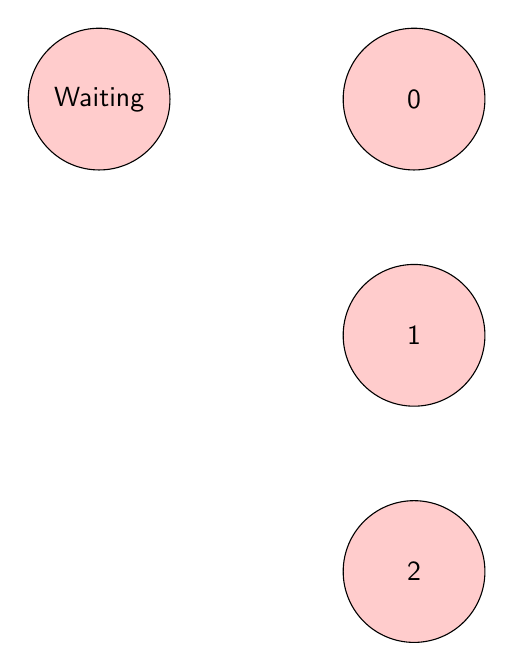
\begin{tikzpicture}[umlstate/.style={
    circle,
    draw,
    minimum size=1.8cm,
    fill=red!20,
    font=\sffamily
}]

\node[umlstate] (Waiting) at (-2,0) {Waiting};
\node[umlstate] (zero) at (2,0) {0};
\node[umlstate] (one) at (2,-3) {1};
\node[umlstate] (two) at (2,-6) {2};

\umltrans[arg=graspAt,pos=0.5]{Waiting}{zero}
\umltrans[arg=notifyEnd,pos=0.5]{zero}{one}
\umltrans[arg=notifyEnd,pos=0.5]{one}{two}
\umltrans[arg=notifyEnd,pos=1.5,arm1=3cm,geometry=-|-]{two}{zero}

\end{tikzpicture}
\end{center}
\end{figure}

Por lo tanto, el estado \textit{Waiting} no implementa \verb|notifyOrder|, mientras que los estados 0, 1 y 2 no implementan \verb|graspAt|. En cambio, \textit{Waiting} sí implementa \verb|graspAt|, el cual calcula los pasos y ejecuta el primero utilizando el iterador. Posteriormente, por cada \verb|notifyEnd| los subsistemas informan al \MainController que finalizaron la ejecución de la orden, y en cada notificación se transiciona a un nuevo estado. Una vez ejecutado \verb|graspAt|, se transiciona al estado 0; al recibir un \verb|notifyEnd| se pasa al estado 1, y de la misma forma hasta llegar al estado 2. Cuando se está en el estado 2 y se recibe un \verb|notifyEnd|, lo que ocurre es que se ejecuta un nuevo paso si aún quedan pasos en el iterador; en caso contrario, se transiciona nuevamente a \textit{Waiting}, dado que la secuencia de ejecución ha finalizado.

Está claro que, para poder sostener este comportamiento, los subsistemas deben responder a estas necesidades. Es decir, cada uno debe invocar el método \verb|notifyEnd| del \MainController como un \textit{callback} cuando realmente hayan terminado de ejecutar la orden, es decir, cuando alcanzan el \textit{set-point}. Los subsistemas son los encargados de determinar cuándo un paso se completó. En el caso de aquellos que requieren un seguimiento exhaustivo, al llegar al \textit{set-point} se transiciona del estado \textit{Moving} al estado \textit{Waiting}; en ese punto se puede incluir la llamada a \verb|notifyEnd|, como ocurre en el método \verb|moving| del módulo \Moving. En el caso del subsistema de la pinza, que no requiere seguimiento, la llamada puede agregarse inmediatamente después de aplicar el cambio en el módulo \Pinza.

\subsubsection*{Conclusión}

La solución propuesta mejora varios aspectos a la que utiliza como critério de división la funcionalidad. Por un lado, se anticipa a cambios probables tales como los de la tabla \ref{tablaConclu}.

\begin{table}[H]
\centering
\caption{Anticipos al cambio del diseño propuesto para el brazo robótico.}
\label{tablaConclu}
\resizebox{\textwidth}{!}{%
\begin{tabular}{|p{3cm}|p{5cm}|p{8cm}|}
\hline
\textbf{Item de cambio}    & \textbf{Naturaleza del cambio}  & \textbf{Manejo del cambio}  \\ \hline
\textbf{Hardware}          &  
    - Agregar, quitar o modificar actuadores y sensores.
    
    - Cambios en la comunicación.
&  
Los subsistemas están desacoplados del control principal, permitiendo agregar, quitar o modificar componentes de manera independiente respetando las interfaces definidas.  
La modularización permite gestionar sensores, actuadores y comunicación por separado. La lógica de control puede modificarse fácilmente cambiando la implementación del módulo Algoritmo.
\\ \hline
\textbf{Lógica de control} &  
    - Cambios en decisiones de trabajo, como ejecución secuencial o criterios de avance.
&  
El comportamiento está encapsulado en módulos. La máquina de estados que controla la ejecución puede modificarse fácilmente agregando o editando estados en el iterador Steps.  
\\ \hline
\end{tabular}
}
\end{table}

Además, se fomenta la reutilización del código, permitiendo aplicar las soluciones existentes a distintos problemas. Cualquier modificación futura requerirá menos esfuerzo por parte de los desarrolladores, ya que el sistema será más fácil de comprender. La documentación también contribuye a esta facilidad de mantenimiento. Los cambios probables están encapsulados, por lo que el control de calidad se reduce a verificar módulos individuales y no secciones de código enteras.

